%%==================================================
%% diss.tex for SJTU Master Thesis
%% based on CASthesis
%% modified by wei.jianwen@gmail.com
%% version: 0.3a
%% Encoding: UTF-8
%% last update: Dec 5th, 2010
%%==================================================

% 字号选项: c5size 五号(默认) cs4size 小四
% 双面打印(注意字号设置)
\documentclass[cs4size, a4paper, twoside]{sjtuthesis} 
% 单面打印(注意字号设置)	
% \documentclass[cs4size, a4paper, oneside, openany]{sjtuthesis} 

% \usepackage[sectionbib]{chapterbib}%每章都用参考文献

\newboolean{DOIT}
\setboolean{DOIT}{false}%编译某些只想自己看的内容,编译true,否则false

%% 行距缩放因子(x倍字号)
\renewcommand{\baselinestretch}{1.3}

% 设置图形文件的搜索路径d
\graphicspath{{figure/}{figures/}{logo/}{logos/}{graph/}{graphs}}

%%========================================
%% 在sjtuthesis.cls中定义的有用命令
%%========================================
% \cndash 中文破折号
% 数学常量
% \me 对数常数e
% \mi 虚数单位iv
% \mj 虚数单位j
% \dif 直立的微分算符d为直立体。
% 可伸长的数学箭头、等号
% \myRightarrow{}{}
% \myLeftarrow{}{}
% \myBioarrow{}{}
% \myLongEqual{}{}
% 参考文献
% \upcite{} 上标引用
%%========================================


\begin{document}

%%%%%%%%%%%%%%%%%%%%%%%%%%%%%% 
%% 封面
%%%%%%%%%%%%%%%%%%%%%%%%%%%%%% 

% 中文封面内容(关注内容而不是形式)
\title{数据库驱动认知无线电网络中的隐私保护}
\author{张\quad{}龙}
\advisor{朱浩瑾 \ 副教授}
\degree{硕士}
\defenddate{2015年1月}
\school{上海交通大学}
\institute{电子信息与电气工程学院}

\studentnumber{1120339081}
\major{计算机科学与技术}

% 英文封面内容(关注内容而不是表现形式)
\englishtitle{Privacy Preservation in Database-driven Cognitive Radio Networks}
\englishauthor{\textsc{Long Zhang}}
\englishadvisor{Asso. Prof. \textsc{Haojin Zhu}}
\englishschool{Shanghai Jiao Tong University}
\englishinstitute{\textsc{School of Electronic Information and Electric Engineering} \\
  \textsc{Shanghai Jiao Tong University} \\
  \textsc{Shanghai, P.R.China}}
\englishdegree{Master}
\englishmajor{Computer Science and Technology}
\englishdate{Jan. 2015}

% 封面
\maketitle

% 英文封面
\makeenglishtitle

% 论文原创性声明和使用授权
\makeDeclareOriginal
\makeDeclareAuthorization

%%%%%%%%%%%%%%%%%%%%%%%%%%%%%% 
%% 前言
%%%%%%%%%%%%%%%%%%%%%%%%%%%%%% 
\frontmatter

% 摘要
%%==================================================
%% abstract.tex for SJTU Master Thesis
%% based on CASthesis
%% modified by wei.jianwen@gmail.com
%% version: 0.3a
%% Encoding: UTF-8
%% last update: Dec 5th, 2010
%%==================================================

\begin{abstract}

认知无线电网络用于解决频谱固定分配政策导致的无线频谱资源的浪费,它允许认知用户使用其物理范围内未占用的频谱资源(频谱空洞)从而提高无线频谱的利用率。传统认知无线电网络通过频谱感知来确定可用频谱信息。联邦通信委员会近期提出了数据库驱动认知无线电网络的概念,允许使用数据库查询作为频谱感知的替代方法来获取可用频谱信息。它把可用频谱获取的任务从终端用户转移到中心数据库,使得用户能够获得更准确的频谱信息,而且大大简化了系统部署的复杂度。
在数据库驱动认知无线电网络的频谱查询过程中,认知用户和数据库交互的数据与用户位置存在一定的相关性,导致网络中的主用户和认知用户都存在位置隐私和轨迹隐私泄露的风险。本文发现在数据库驱动认知无线电网络中,数据库能够根据认知用户的频谱使用信息来推测其位置,同时认知用户也能够根据收集到的可用频谱信息来推断网络中主用户的位置。本文分别提出了针对静止用户和移动用户的攻击方法。对于静止用户,我们提出一种通用的位置推断攻击方法,主用户和认知用户的位置都能够被对方锁定在一个较小的区域范围内。对于移动用户,数据库也可以根据收集到的频道注册信息实施一种基于概率的轨迹跟踪攻击。为抵御在频谱查询过程中的用户位置隐私泄露,本文提出一种改进的隐私保护的频谱查询方式,认知用户在频谱请求阶段通过查询临近区域的方式来模糊自身位置,并基于这些信息进行频道选择。数据库在提供可用频谱阶段也将主用户位置进行模糊处理来增加推断攻击的不确定性。最后,认知用户对隐私保护程度进行权衡并选择最大程度上实现隐私保护的频道。本文将提出的攻击方法和隐私保护方法进行仿真测试,实验结果证明所提出的隐私保护方案可以很大程度上提高数据库驱动认知无线电网络中的用户位置隐私。

  \keywords{\large 认知无线电网络 \quad 位置隐私 \quad 轨迹隐私 \quad 可用频谱查询 \quad 隐私保护}
\end{abstract}

\begin{englishabstract}

The concept of Cognitive Radio Networks (CRNs) was first proposed in 1999. It is considered to solve the problem of wireless spectrum wastage under the paradigm of fixed spectrum allocation. In CRNs, unregistered users (secondary users) can search and access the unoccupied spectrum (spectrum hole) temporarily to enhance the spectrum utilization of wireless spectrum. In traditional CRNs, secondary users should have to implement spectrum sensing to determine the available spectrum. Federal Communication Committee (FCC) proposed database-driven CRNs, in which secondary users could obtain available spectrum via querying the database instead of spectrum sensing based on the pre-established channel. Database-driven CRNs shifts the function of available spectrum retrieval from terminal devices to the central database and enable secondary users to obtain more accuracy available spectrum information and in the meaning time, simplify the deployment of the networks. 
In database-driven CRNs, secondary users get the available spectrum information via the process of spectrum query. In the process spectrum query, since the communication contents between secondary users and the database are correlated with the locations of primary users and secondary users, there are threats of privacy leaking. In this article, we identify that the database is able to infer the locations of secondary users based on the utilized channels of secondary users. On the other hand, secondary users could also infer the locations of primary users based on the spectrum availability information. For fixed users, we proposed a general location inference attack scheme, based on which the primary users and secondary users could be localized in a relative small area. For mobile secondary users, the database could also launch probabilistic tracking attack based on the collected information of channel utilization. To thwart the location and trajectory privacy leaking in spectrum query, we proposed an improved privacy preserving spectrum query scheme, in which secondary users obfuscate the submitted location, which could also be utilized to help determine the best channel. Then the database perturbs the locations of primary users before calculating the available spectrum information. Finally, secondary users estimate the location privacy level to determine the selected channel. We conduct experiments to verify the proposed location inference attacks and location protection schemes. The results of the experiments show that the privacy preserving schemes significantly improve the users’ location privacy and trajectory privacy in database-driven CRNs.

  \englishkeywords{\large Cognitive Radio Networks, Location Privacy, Trajectory Privacy, Available Spectum Query, Privacy Preserving}
\end{englishabstract}


% 目录
\tableofcontents
% 插图索引
\listoffigures
\addcontentsline{toc}{chapter}{\listfigurename} %将图索引加入全文目录
%% 表格索引
%\listoftables
%\addcontentsline{toc}{chapter}{\listtablename}  %将表格索引加入全文目录

% 主要符号、缩略词对照表
%%==================================================
%% symbol.tex for SJTU Master Thesis
%% based on CASthesis
%% modified by wei.jianwen@gmail.com
%% version: 0.3a
%% Encoding: UTF-8
%% last update: Dec 5th, 2010
%%==================================================

\chapter{主要符号对照表}
\label{chap:symb}
\begin{tabular}{ll}

 \hspace{2em}$DB$       & \hspace{5em}数据库 \\
 \hspace{2em}$SU$       & \hspace{5em}认知用户 \\
 \hspace{2em}$PU$ \qquad     & \hspace{5em}主用户 \\
 \hspace{2em}$ch$       & \hspace{5em}频道 \\
 \hspace{2em}$P$ \qquad     & \hspace{5em}功率 \\
 \hspace{2em}$d$       & \hspace{5em}距离 \\




\end{tabular}


%%%%%%%%%%%%%%%%%%%%%%%%%%%%%% 
%% 正文
%%%%%%%%%%%%%%%%%%%%%%%%%%%%%% 
\mainmatter


%% 各章正文内容
%%==========================
%% chapter01.tex for SJTU Master Thesis
%% based on CASthesis
%% modified by wei.jianwen@gmail.com
%% version: 0.3a
%% Encoding: UTF-8
%% last update: Dec 5th, 2010
%%==================================================

%\bibliographystyle{sjtu2} %[此处用于每章都生产参考文献]
\chapter{研究背景}
\label{chap:introduction}



%\section{数据库驱动认知无线电网络}

无线网络凭着它各方面的优点,越来越受到人们的关注。当前无线网络已经表现出迅猛的发展势头,不仅是在企业中,还包括家庭、公共接入和嵌入式设备市场等。无线网络正在改变着人们的种种观念以及生活方式。市场研究公司ABI Research于2013年发布的统计数据显示,全球物联网上的无线联网设备总数已经突破100亿台,预计2020年将达到300亿台,而且这个数字还在持续迅速增长。随着智能手机以及各种无线应用的发展,无线频谱资源正面临着前所未有的紧迫需求。当前对无线频谱的管理采用固定分配的政策,30MHz$\sim$3GHz的无线频段都已分配给固定的无线业务。美国联邦通信委员会(Federal Communication Commission, FCC)的资料显示,当前实际环境中无线频谱的使用情况随着时间和地理位置发生变化,其频谱利用率的时间和空间变化率可达$15\% \sim 85\%$\cite{akyildiz2006next}。大部分固定分配的无线频谱资源的时间利用率和空间利用率非常低,这直接导致稀缺的无线频谱资源变得更加紧张。

Joseph Mitola博士于1999年提出了认知无线电的概念\cite{mitola1999cognitive}。他指出认知无线电是一种智能化的软件无线电,是更灵活的的软件无线电。认知无线电是一种智能频谱共享技术,“认知”意味着网络具有对周围无线频谱的感知能力,即能够嗅探其所处空间周围的无线频谱使用情况,发现一定时间空间范围内的空闲频谱(频谱空洞)。认知无线电网络中的用户设备能够对获取的信息进行处理和学习,从而进行动态智能决策。认知无线电的实现基于软件无线电的可编程性,在发现频谱空洞时可以智能调整通信参数,从而伺机使用这些临时未被使用的频谱。认知无线电技术现在已经被学术界和工业界公认为解决无线频谱资源匮乏问题的最佳手段。认知无线电网络中有两种用户:主用户和认知用户。主用户是频谱注册用户,是频谱的合法所有者,可以无条件使用无线电管理部门已预先分配的频谱资源,对已申请频谱资源具有排他的使用权。认知用户没有固定的频谱使用权,只能通过对其周围环境中的频谱使用情况进行学习并发现频谱空洞,才能伺机利用这些频谱空洞伺机进行通信。主用户对无线频谱使用的排他性是指在一定的保护范围内,认知用户不允许接入网络,以免其发射信号对主用户造成干扰。认知无线电网络的典型结构如图\ref{fig:crn}所示。

\begin{figure}[!htp]\label{fig:crn}
  \centering
  \includegraphics[width=0.8\textwidth]{figures/chap1/crn}\bicaption[fig:crn]{认知无线电网络组网结构}{认知无线电网络组网结构}{Fig}{Architecture of Cognitive Radio Networks}
\end{figure}

认知无线电网络应该具备以下功能模块\cite{akyildiz2006next}:

(1)频谱感知:认知用户设备必须具备比较准确的感知无线频谱的能力,能够在相应的频段内进行频谱检测,识别频谱空洞,在保证不干扰主用户的前提下使用频谱;

(2)频谱管理:网络能够捕获最佳的信道,从而满足用户对频谱资源质量的要求;

(3)频谱移动:为避免对主用户造成干扰,认知用户设备必须具备在不同频段的频谱资源之间实现无缝切换的能力;

(4)频谱共享:在存在多个用户设备时,网络能够为所有认知用户设备提供一个公平的频谱资源调度。

其中感知功能是认知无线电网络中的关键环节,是认知无线电网络能够实现的前提条件。当前比较流行的频谱感知技术主要有能量感知和特征检测等。能量感知的优点是速度快,但精确度不是很高;与之相反,特征检测的精确度相对比较高但是运行速度较慢。由于单个用户的感知结果可能会因为遮挡、衰落等原因与实际频谱占用情况有偏差,因此为提高频谱感知的精确性,研究者提出合作感知机制,即网络中每个用户设备先进行独立感知,然后若干用户将感知结果上报给融合中心进行计算并确定最终的可用频谱。这是当前主流的频谱感知方式,但它在大大提高了频谱感知精确性的同时,也引入了一些严重的安全和隐私问题。关于合作频谱感知的安全问题,已有大量研究者进行了研究。目前提出的主要的安全威胁主要有:

(1)模仿主用户攻击:攻击者在信道上发送与主用户特征相同的信号,导致其他认知用户误以为主用户存在,因此认知用户将此数据信道判定为不可用,无法使用该信道,导致频谱资源浪费。

(2)阻塞攻击:由于无线信道中的广播特性,攻击者可以随机或有针对性地选择某些可用信道进行阻塞,从而导致认知用户无法利用空闲信道进行正常通信。

(3)频谱感知数据篡改攻击:攻击者向邻居节点或融合中心发送错误的本地频谱感知信息,导致接收者做出错误的频谱感知判断结果,进而可能导致对主用户造成干扰。

(4)虚假申请攻击:恶意的认知用户通过对信道的申请,获得信道临时使用权后,却并不使用此信道。这种行为严重增加了网络负载并造成资源浪费。

由于合作频谱感知涉及的环节较多,硬件成本以及计算复杂度较高,同时感知结果的精确度还比较依赖环境和一些人为因素,因此不太适合在现实中大规模部署。


一种可供替代的实现认知无线电网络的机制是数据库驱动认知无线电网络(Database-driven CRNs)。FCC于2008年首次公布关于数据库驱动认知无线电网络的提议并于2012年首次发布了关于数据库驱动认知无线电的相关规定,明确声明取消认知无线电网络用户必须具备频谱感知能力的限制。在数据库驱动认知无线电网络中,每个辖区范围内设定一个中心数据库服务器,辖区内的认知用户只要向数据库提交地理位置信息即可获取该位置的可用频谱。FCC指定了包括Google Inc.等九个公司作为数据库的管理者。据报道,Koos Technical Services Inc.和Telecodia Technologies Inc.两家公司已经获得FCC批准并已实现了数据库运营。与之前所述的传统认知无线电技术相比,数据库驱动认知无线电使用数据库查询方式取代了频谱感知来获取可用频谱信息,将频谱学习的复杂功能从用户终端中剥离并转移至中心数据库。这种简单的可用频谱获取方式具有更好的准确性和易用性,更适合在现实中部署,因此一经提出便迅速得到了政府和工业界的认可。数据库驱动认知无线电网络要求每个认知用户接入中心数据库并根据位置来查询可用频谱。中心数据库负责生成和维护其服务范围内的可用频谱信息。认知用户的可用频谱查询过程基于预先建立的Internet连接,由安全套接层/传输层安全协议(SSL/TLS)负责保证网络传输层以下的信息安全。


从网络安全的角度考虑来讲,在数据库驱动认知无线电网络中,大部分传统认知无线电网络合作频谱感知过程中存在的攻击都可以避免。尽管如此,数据库驱动认知无线电网络仍然带来了新的安全问题。网络中的可用频谱信息由数据库根据网络中用户的分布和较为复杂的环境因素计算得到。因此,可用频谱信息与网络中用户的位置具有一定的相关性,对可用频谱信息的分析可能导致用户位置隐私的泄露。近年来,人们对隐私保护的关注度越来越高,因此隐私问题一直是很多领域相关研究工作中的重点。在无线网络中,由于其广播的特性,使得潜在的攻击者能够很容易地获取通信过程中的数据并进行分析从而危害用户的隐私安全。近年来,随着各种无线应用的飞速发展,给人们使用网络服务带来了很大方便,但与此同时,其隐私保护方面的形势也越来越严峻。尤其在近年来发展迅速的基于位置服务(Location Based Service, LBS)系统中,用户根据所处位置获得相应服务,这使得用户的位置隐私直接暴露在外,甚至用户所经历的时空轨迹都有可能被攻击者非法获取。更进一步,用户的位置隐私与其他方面隐私密切相关,位置隐私泄露将会直接导致更严重的其他方面的隐私泄露。数据库驱动认知无线电网络是LBS的一种应用形式,网络中有两类用户:固定用户和移动用户,其中移动用户又分为第一类移动用户和第二类移动用户。第二类移动用户具备定位和直接接入数据库的能力,第一类移动用户不具备定位和直接接入数据库的能力,只能向周围的第二类移动用户或固定用户查询可用频谱。无论固定用户还是移动用户,都同样面临着传统LBS中存在的隐私泄露风险。具体地讲,固定的认知用户需要提交精确地理位置才能获得准确的可用频谱信息,数据库可以直接获取认知用户的位置,即使通过适当的手段将认知用户位置信息隐藏\cite{gao2013location},数据库还是可以通过认知用户的频谱使用记录和频谱的覆盖范围来推测认知用户的位置。与此同时,由于数据库提供的可用频谱信息与网络中主用户的位置具有较大的相关性,恶意的认知用户还能够根据其收集到的可用频谱信息对主用户进行位置推断攻击。此外,对于网络中移动的认知用户,由于其在运动轨迹上所经历的可用频谱以及使用过的频谱与轨迹信息具有同样的相关性,因此也面临着一定的轨迹隐私泄露风险。传统的LBS中的隐私保护方式无法直接应用与数据库驱动认知无线电场景中,因为相比其他LBS应用而言,数据库驱动认知无线电网络中对用户提交的地理位置要求更严格,一般要求定位误差小于50米,而且要求每个认知用户具有唯一不变的身份标识,因此如何保护用户的位置和轨迹隐私是一个具有挑战性的问题。我们将在第二章对相关领域的研究工作进行简要总结并在后续章节对数据库驱动认知无线电网络中的位置隐私和轨迹隐私的研究工作进行详细论述。




%现在,交大学位论文 \LaTeX 模板的代码在github上维护,地址是:
%
%	\url{https://github.com/weijianwen/sjtu-thesis-template-latex/}



%\begin{itemize}
%	\item \href{https://github.com/weijianwen/sjtu-thesis-template-latex/archive/bachelor-0.5.3.zip}{交大学士学位论文模板\version} 
%	\item \href{https://github.com/weijianwen/sjtu-thesis-template-latex/archive/master-0.5.3.zip}{交大硕士学位论文模板\version}
%	\item \href{https://github.com/weijianwen/sjtu-thesis-template-latex/archive/phd-0.5.3.zip}{交大博士学位论文模板\version}
%\end{itemize}
%
%欢迎大家使用交大学位论文模板!你可以通过如下的途径反馈模板使用过程中遇到的问题:\href{https://github.com/weijianwen/sjtu-thesis-template-latex/issues}{开issue}
%\href{https://bbs.sjtu.edu.cn/bbsdoc?board=TeX_LaTeX}{水源LaTeX版}发帖,或者是给\href{mailto:weijianwen@gmail.com}{我}发送邮件---你可能需要好几天才能收到我的邮件回复。
%
%
%
%\label{sec:features}
%
%这个模板使用的中文解决方案是 \XeTeX/\LaTeX 。
%参考文献使用BibTeX处理,可以生成符合国标GBT7714风格的参考文献列表。
%模板在Windows,Linux和Mac OS X下测试通过,更详细的系统要求请参考\ref{sec:requirements}。
%
%模板的外观表现和功能都放在sjtuthesis.cls和sjtuthesis.cfg中,在对外观进行细微调整时,只需要更新这两个文件,不需要对.tex源文件做修改。
%
%最后,给出一个列表,罗列一下这个模板的功能要点:
%
%\begin{itemize}
%\item 使用 \XeTeX 引擎处理中文;
%\item 包含中文字符的源文件(.tex, .bib, .cfg),编码都使用UTF-8;
%\item 使用BibTeX处理参考文献。参考文献表现形式(格式)受.bst控制,方便在不同风格间切换,目前生成的列表符合国标GBT7714要求;
%\item 可以直接插入EPS/PDF/JPG/PNG格式的图像,并且\emph{不需要}bounding box文件(.bb)。
%\item 模板的格式受sjtumater-xetex.cls和sjtuthesis.cfg控制,方便模板更新和模板修改。
%\end{itemize}
%
%\subsection{系统要求}
%\label{sec:requirements}
%
%要使用这个模板协助你完成研究生学位论文的创作,下面的条件必须满足:
%
%\begin{itemize}
%\item 操作系统字体目录中有TeX Gyre Termes西文的:Regular, Italic, Bold, Bold Italic四种OTF字体\footnote{TeX Gyre Termes字体可以从\href{http://www.gust.org.pl/projects/e-foundry/tex-gyre/termes}{http://www.gust.org.pl/projects/e-foundry/tex-gyre/termes}下载。我也附带了一份TeX.Gyre.Termes.Fonts.zip在模板中,解压缩到字体目录后用fc-cache -fv刷新即可,用fc-list应该能看到。};
%\item 操作系统字体目录中有AdobeSongStd、AdobeKaitiStd、AdobeHeitiStd、AdobeFangsongStd四款中文字体\footnote{Adobe这四款中文OTF字体可以从Adobe Reader安装目录拿到。};
%\item \TeX 系统有 \XeTeX 引擎;
%\item \TeX 系统有ctex宏包;
%\item 你有使用 \LaTeX 的经验。
%\end{itemize}
%
%你可以试着编译模板文件夹中自带的test.tex文件,看看你的 \TeX 系统是否满足上面的要求:
%
%\begin{lstlisting}[basicstyle=\small\ttfamily, caption={编译测试文件test.tex}, numbers=none]
%xelatex test.tex
%\end{lstlisting}
%
%如果编译出的test.pdf中能够:显示中英文内容、显示4幅图像、正确嵌入AdobeSongStd和TeXGyreTermes字体(通过PDF阅读器的“属性”查看)、并且看到了英文字符的连字(ligature)和\textsc{SmallCapital}特性,那么恭喜你,你的 \TeX 系统应该能够编译这个学位论文模板。
%
%目前,我在手头的几个 \TeX 环境上都做过测试,MacTeX 2011, TeXLive 2011和C\TeX 2.9都能够顺利编译。在你到版上抱怨模板不能工作前,请确定你的 \TeX 系统能够编译前面的test.tex文件。欢迎大家到\href{https://bbs.sjtu.edu.cn/bbsdoc?board=TeX_LaTeX}{水源LaTeX版}反馈问题。为了提高解决问题的速度,请在帖子中说明:是否顺利编译模板、错误提示、操作系统版本、\TeX 系统版本和最近对 \TeX 系统做的操作(如升级等)。
% 
%\subsection{模板文件布局}
%\label{sec:layout}
%
%\begin{lstlisting}[basicstyle=\small\ttfamily,caption={模板文件布局},label=layout,float,numbers=none]
%  |-- diss.tex
%  |-- README.pdf
%  |-- sjtuthesis.cfg
%  |-- sjtuthesis.cls
%  |-- body
%  |   |-- abstract.tex
%  |   |-- app1.tex
%  |   |-- app2.tex
%  |   |-- chapter01.tex
%  |   |-- chapter02.tex
%  |   |-- conclusion.tex
%  |   |-- projects.tex
%  |   |-- pub.tex
%  |   |-- resume.tex
%  |   |-- symbol.tex
%  |   \-- thanks.tex
%  |-- figures
%  |   \-- chap2
%  |-- GBT7714-2005NLang.bst
%  |-- Makefile
%  |-- reference
%  |   |-- chap1.bib
%  |   \-- chap2.bib
%  |-- test.tex
%  \-- test.pdf
%\end{lstlisting}
%
%你拿到手的模板文件大致会包含代码\ref{layout}所列的文件,乍看起来还是挺令人头大的。
%并且,这还是“干净”的时候,等到真正开始处理的时候,会冒出相当多的“中间文件”,这又会使情况变得更糟糕。
%所以,有必要对这些文件做一些简要说明。
%看完这部分以后,你应该发现,其实你要关心的文件类型并没有那么多。
%
%\subsubsection{格式控制文件}
%\label{sec:format}
%
%格式控制文件控制着论文的表现形式,包括以下几个文件:
%sjtuthesis.cfg, sjtuthesis.cls和GBT7714-2005NLang.bst。
%其中,``.cfg''和``.cls''控制论文主体格式,``.bst''控制参考文献条目的格式,
%
%一般用户最好``忽略''格式控制文件的存在,不要去碰它们。
%有其他格式需要,欢迎到板上发贴。
%对于因为擅自更改格式控制文件出现的问题,我不一定能够解决。
%
%\subsubsection{主控文件diss.tex}
%\label{sec:disstex}
%
%主控文件diss.tex的作用就是将你分散在多个文件中的内容``整合''成一篇完整的论文。
%使用这个模板撰写学位论文时,你的学位论文内容和素材会被``拆散''到各个文件中:
%譬如各章正文、各个附录、各章参考文献等等。
%在diss.tex中通过``include''命令将论文的各个部分包含进来,从而形成一篇结构完成的论文。
%封面页中的论文标题、作者等中英文信息,也是在diss.tex中填写。
%部分可能会频繁修改的设置,譬如行间距、图片文件目录等,我也放在了diss.tex中。
%你也可以在diss.tex中按照自己的需要引入一些的宏包
%\footnote{我对宏包的态度是:只有当你需要在文档中使用那个宏包时,才需要在导言区中用usepackage引入该宏包。如若不然,通过usepackage引入一大堆不被用到的宏包,必然是一场灾难。由于一开始没有一致的设计目标,\LaTeX 的各宏包几乎都是独立发展起来的,因重定义命令导致的宏包冲突屡见不鲜。}
%。
%
%大致而言,在diss.tex中,大家只要留意把``章''一级的内容,以及各章参考文献内容包含进来就可以了。
%需要注意,处理文档时所有的操作命令 \cndash{} xelatex, bibtex等,都是作用在diss.tex上,而\emph{不是}后面这些``分散''的文件,请参考\ref{sec:process}小节。
%
%\subsubsection{论文主体文件夹body}
%\label{sec:thesisbody}
%
%这一部分是论文的主体,是以``章''为单位划分的。
%
%正文前部分(frontmatter):中英文摘要(abstract.tex)。其他部分,诸如中英文封面、授权信息等,都是根据diss.tex所填的信息``画''好了,
%不单独弄成文件。
%
%正文部分(mainmatter):自然就是各章内容chapter\emph{xxx}.tex了。
%
%正文后的部分(backmatter):附录(app\emph{xx}.tex);致谢(thuanks.tex);攻读学位论文期间发表的学术论文目录(pub.tex);个人简历(resume.tex)。
%参考文献列表是``生成''的,也不作为一个单独的文件。另外,学校的硕士研究生学位论文模板中,也没有要求加入个人简历,所以我没有在diss.tex中引入resume.tex。
%
%\subsubsection{图片文件夹figures}
%\label{sec:figuresdir}
%
%figures文件夹放置了需要插入文档中的图片文件(PNG/JPG/PDF/EPS),建议按章再划分子目录。
%
%\subsubsection{参考文献数据库文件夹reference}
%\label{sec:bibdir}
%
%reference文件夹放置的是各章``可能''会被引用的参考文献文件。
%参考文献的元数据,例如作者、文献名称、年限、出版地等,会以一定的格式记录在纯文本文件.bib中。
%最终的参考文献列表是BibTeX处理.bib后得到的,名为diss.bbl。
%将参考文献按章划分的一个好处是,可以在各章后生成独立的参考文献,不过,现在看来没有这个必要。
%关于参考文献的管理,可以进一步参考第\ref{chap:example}章中的例子。
%
%\subsection{如何使用模板}
%\label{sec:process}
%
%模板的 \LaTeX 源文件需要用 \XeTeX 编译产生PDF文件。
%我在此给出三种命令行下的编译方式:逐行手工执行、使用脚本、使用latexmk,大家可以根据自己的喜好,选择\emph{其中一种}完成工作。
%
%\subsubsection{逐行手工执行}
%
%模板使用 \XeTeX 引擎提供的xelatex的命令处理,作用于“主控文档”diss.tex。并且,可以省略扩展名。
%在命令提示符下逐行敲入如下命令完成编译。
%
%\begin{lstlisting}[basicstyle=\small\ttfamily, caption={手动执行编译过程}, numbers=none]
%xelatex -no-pdf --interaction=nonstopmode diss
%bibtex diss 
%xelatex -no-pdf --interaction=nonstopmode diss 
%xelatex --interaction=nonstopmode diss 
%\end{lstlisting}
%
%运行bibtex的时候会提示一些错误,猜测是{{\sc Bib}\TeX}对UTF-8支持不充分,一般不影响最终结果。留意因为拼写错误导致的``找不到文献错误''即可。
%
%基本处理流程就是这样,一些 \LaTeX 排版的小例子可以参考第二章。
%
%\subsubsection{使用脚本}
%
%为方便使用,我把上面几条命令放到了两个脚本文件中。
%Linux用户可以使用run.sh脚本,Windows用户可以使用run.bat。
%
%\subsubsection{使用GNU make编译}
%
%模板自带了一个简单的Makefile,使用make可以方便地完成相应任务,如 pdf, view, clean, distclean等。
%
%\begin{lstlisting}[basicstyle=\small\ttfamily, caption={使用GNU make编译}, numbers=none]
%make && make view
%\end{lstlisting}
%
%\section{从 \CJKLaTeX 转向 \XeTeX}
%\label{sec:whydvipdfm}
%
%我习惯把v0.2a使用dvipdfmx编译的硕士学位论文模板称为``\CJKLaTeX 模板'',而这个使用 \XeTeX 引擎(xelatex程序)处理的模板则被称为``\XeTeX/\LaTeX 模板''。
%从 \CJKLaTeX 模板迁移到 \XeTeX\LaTeX 模板的好处有下:
%\begin{enumerate}
%\item[\large\smiley] 搭建 \XeTeX 环境比搭建 \CJKLaTeX 环境更容易;
%\item[\large\smiley] 更简单的字体控制;
%\item[\large\smiley] 完美支持PDF/EPS/PNG/JPG图片,不需要``.bb''文件;
%\item[\large\smiley] 支持OpenType字体的复杂字型变化功能(通常只有字母字体才有,学术文章也暂时用不上);
%\end{enumerate}
%
%当然,这也是有代价的。由于 \XeTeX 比较新,在我看来,使用 \XeTeX 模板所必须付出的代价是:
%
%\begin{enumerate}
%\item[\large\frownie] 必须把你“古老的” \TeX 系统更新为较新的版本。TeXLive 2012和CTeX 2.9.2能够编译这份模板,而更早的版本则无能为力。
%\item[\large\frownie] 需要花一些时间把你在老模板上的工作迁移到新模板上。
%\end{enumerate}
%
%第一条就看你如何取舍了,新系统通常意味着更好的兼容性,值得升级。而转换模板也不是什么特别困难的事情,可以这样完成:
%
%\begin{enumerate}
%\item 备份你要转换的源文件,以防你的工作成果丢失;
%\item 将你原来的``.tex''和``.bib''文件"另存为"UTF-8编码的文件。iconv、vim、emacs、UEdit等等工具都可以完成。WinEdt对文件编码识别功能很差(到了v6.0还是如此),不推荐作为字符编码转换工具;
%\item 将diss.tex导言区中的内容替换为XeTeX模板diss.tex导言区的内容;
%\item 将你对原先导言区的修改,小心翼翼地``合并''到新的导言区中;
%\item 使用XeTeX模板中的GBT7714-2005NLang.bst替换原有的bst文件,新的bst文件只是将字符编码转换为UTF--8。
%\item 删除bouding box文件``.bb'';
%\item 使用本文\ref{sec:process}介绍的方法,重新编译文档;
%\end{enumerate}
%
%\section{硕士学位论文格式的一些说明}
%\label{sec:thesisformat}
%
%所有关于研究生学位论文模板的要求,我参考的都是下面这个教务处的网址
%\href{http://www.gs.sjtu.edu.cn/policy/fileShow.ahtml?id=130}{《上海交通大学研究生学位论文格式的统一要求 》}。
%
%可惜,这个网址没有给出具体可用的“模板文件”。
%并且,``要求''中的一些要求也不仅合理,譬如,公式和公式编号之前要用……连接,实现起来困难,看起来也不美观,从来没有人这样用,所以无视之。
%师兄师姐的学位论文也是我可以参考的“范本”,尽管这些范本也不是很规范。
%我希望制作出的这个学位论文模板尽可能符合教务处的要求,如果有任何建议,欢迎提出!
%
%这个模板是为``双面打印''准备的,也就是说,迎面页总是奇数页,新的一章将从奇数页开始,``迎面页''和``背面页''(或者说奇数页和偶数页)的左右页眉是相互颠倒的,奇数页和偶数页的左右页边距也会被颠倒。通过双面打印得到的学位论文就像一本正常的书。
%
%你可以将diss.tex中设定文档类的语句改为:
%
%\begin{quote}
%  {\scriptsize\verb+\documentclass[cs4size, a4paer, cs4size, oneside, openany]{sjtuthesis}+}
%\end{quote}
%
%这样,就变成了适合“单面打印”的论文,新的一章可以从偶数页开始。
%
%关于页眉页脚。奇数页页眉为:左边``上海交通大学硕士学位论文'',右边:``章节名'';偶数页页眉为:左边``上海交通大学硕士学位论文'',右边:``论文题目''。每一章的内容按照排书的习惯,均从奇数页开始。
%
%教务处要求参考文献必须符合GBT7714风格,学校明确提出使用这个标准而不是自己拍脑袋想出别的做法,应该算是谢天谢地了。使用这个模板,结合BibTeX,可以很方便地生成符合GB标准的参考文献列表。
%
%\section{模板更新说明}
%\label{sec:update}
%
%我希望这个模板能够成为大家完成学位论文的助手。
%我会在一段时间内(一个月?一年?),继续维护这个模板,修正其中的错误和不理想的地方。
%我还计划向模板中添加常用的``例子'',譬如表格、公式、图片的排版,这也是我知识汇总的。
%完整的更新记录可参考附录A.
%
%不管怎么说,模板更新应该是一件好事。
%如果``新的格式控制文件''产生的效果对你很有吸引力,那么不妨尝试一下。
%应用新的格式控制文件是一件非常简单的事情:
%你只要把原来的sjtuthesis.cls, sjtuthesis.cfg, GBxxx.bst覆盖(建议备份或者使用版本控制系统),重新编译一遍,应该就OK了。
%
%我大力推荐大家使用\href{http://git-scm.com}{git}\cndash{}一个优秀的代码控制系统\cndash{}管理整个学位论文的协作过程。使用git合并(merge)最新版本的模板,是一件非常安全且无痛的工作。
%


%%==================================================
%% chapter02.tex for SJTU Master Thesis
%% based on CASthesis
%% modified by wei.jianwen@gmail.com
%% Encoding: UTF-8
%%==================================================

\chapter{相关工作}\label{chap:related_work}

本文重点关注数据库驱动认知无线电网络中的位置隐私和轨迹隐私问题。认知无线电网络作为一种无线网络体制,面临着所有无线网络存在的安全和隐私问题。此外,数据库驱动认知无线电网络作为一种基于位置的服务,还将面临着传统基于位置服务系统中所固有的位置隐私和轨迹隐私泄露问题。本章将对相关研究领域的研究成果做一概述。数据库驱动认知无线电网络作为一种有应用前景的新兴认知无线电体制,其安全和隐私等问题必将受到越来越多的关注。

\section{数据库驱动认知无线电网络}\label{sec:database-driven}

数据库驱动认知无线电网络的概念提出时间较短,因此当前相关的文献较少,本小节对已有的关于数据库驱动认知无线电网络机制设计方面的文献进行简要描述。文献\cite{gurney2008geo}提出了一个基于地理信息数据库的认知无线电系统,认知用户可以从地理信息数据库中了解到网络中主用户的位置以及相关的环境信息,因此可以根据相关的传输模型计算可用频谱资源。文章指出,由于频谱感知需要设定一个安全的能量阈值,因此导致大量的频谱资源浪费。相比之下,基于地理信息数据库的认知系统可以更准确地获得可用频谱信息。文献\cite{murty2012senseless}提出通过数据库管理射频频谱资源并首次提出了白空间数据库驱动认知无线电网络Senseless,其中所有认知用户通过查询数据库获得广播电视频段的白空间,数据库对主用户和认知用户的状态和参数进行实时更新并基于Longley-Rice传输模型来预测频谱可用性。文献\cite{ying2013exploring}提出了一种室内的白空间数据库驱动认知无线电系统WISER,作者指出在室外和室内有分别超过$50\%$和$70\%$的白空间频谱。该系统在需要的位置上部署若干频谱感知传感器,由数据库收集数据并预测大楼内部的频谱可用情况从而提供给认知用户。文献\cite{zhangvehicle}指出现有的数据库驱动认知无线电网络模型由于传输模型的原因存在信号强度预测不准确的情况。因此作者提出了V-Scope,利用携带频谱感知传感器的公交车系统来收集沿途的无线频谱可用信息并构建频谱信息数据库。Senseless的优点是减轻了频谱测量的开销,但是由于在Longley-Rice模型中只考虑了地形因素,因此在有遮挡时无法精准地表达传输模型。此外,由于系统没有考虑认知用户的发射功率等因素,因此无法预测信道的质量;WISER通过大量传感器收集频谱数据,由于部署成本较高,只适合应用在较小的物理范围内,可扩展性不好。V-Scope集成了Senseless和WISER的优点,综合考虑了各种环境因素,通过广泛收集数据来重新提炼信号传输模型,并且部署容易。但缺点是测量和存储的开销较大。目前,FCC已经批准Google Inc.等厂家作为频谱数据库的运营者。在美国,无线广播电视频段的频谱可用信息已经对外公开公布,用户可以在诸如TVFool等网站查询。这意味着距离数据库驱动认知无线电网络在实际环境中部署又近了一步。

\section{隐私保护}\label{sec:location-privacy}

隐私是关于个人或机构等实体不愿意被外部揭露的信息,比如行为方式、爱好兴趣、健康情况等。一个实际应用系统的隐私保护水平是衡量其系统可行性的一个关键指标。隐私问题一直是学术界的研究重点,已有大量学者做了深入研究。文献\cite{wang2014location}对主流的隐私保护技术进行了总结并大致归为以下几类:匿名(空间隐形)、随机加扰、差分隐私、密码技术等。匿名的主要思路是将若干个用户分成组,然后对组内的用户进行混淆,打乱用户身份和敏感信息的对应关系。$k$-anonymity\cite{sweeney2002k}和$l$-diversity\cite{machanavajjhala2007diversity}是当前主流的两种匿名技术。$k$-anonymity将用户分成若干个混淆组并要求分组内个体数量不少于$k$,即分组内的用户与其他至少$k-1$个用户是不可区分的;$l$-diversity将用户的信息分为准标识符和敏感属性,要求匿名组内的个体被映射到某个敏感属性的概率不超过$1/l$。($\alpha,k$)-anonymity\cite{wong2006alpha}是一种改进的$k$-anonymity机制,综合考虑了$k$-anonymity和$l$-diversity的要求,它除了要求组内用户至少与其他$k-1$个用户不可区分之外,还要求敏感属性在组内出现的频率不超过$\alpha k$。
随机加扰\cite{adam1989security}是一种隐私保护的从个体中提取数据的方法,在诸如合作感知\cite{liu2012cloud}、数据挖掘\cite{du2003using}等许多隐私保护的应用中被广泛采用。其基本思路是用人造的随机数据取代原始的敏感数据,但同时需要保证替换后的数据的某些统计特性与原始数据相同,这种方法能够隐藏真实敏感数据,同时能够保证攻击者无法将隐私数据和用户个体关联起来。
差分隐私\cite{dwork2006differential}是当前比较流行的一种隐私模型,其基本思路是保证移除或增加一条数据记录不会很明显地影响输出结果。差分隐私定义了一个比较严格的攻击模型,对隐私泄露风险给出了定量的表示和证明。差分隐私保护基于数据失真技术,仅通过加入极少量的噪声就能够达到较高的隐私保护效果。差分隐私在学术界引起了较高的关注度。文献\cite{cormode2011differentially}提出针对特定的数据类型,通过简化步骤和降低敏感度等方式解决了稀疏数据在差分隐私保护过程中噪音添加量过大的问题。文献\cite{dwork2010differential}还基于差分隐私的思想提出了隐私保护性能更好的泛隐私概念。文献\cite{li2011provably}还首次提出将差分隐私与$k$-anonymity算法结合并用于解决微数据隐私保护的数据发布问题。
基于密码技术的隐私保护方法涵盖范围比较广,私有信息提取(Private Information Retrieval,PIR)\cite{chor1998private}就是在数据库查询过程中的一种高效的隐私保护方法。在一般的数据库查询过程中,私有信息提取使得用户能够在不暴露查询条目的前提下进行查询,即查询的内容对数据库来说是不可见的。


特别地,随着移动应用的发展,LBS的出现给人们生活带来了极大的便利,同时也使得用户的位置隐私面临严重的泄露风险。在位置隐私保护方面,上述几种通用的数据隐私保护方案或其变种一般都能够取得一定的位置隐私保护效果。此外,针对LBS中的位置隐私泄露问题,学术界已积累了大量的研究成果。文献\cite{freudiger2012evaluating}基于现实中的移动轨迹数据对LBS中的位置隐私进行了量化和评估,说明了LBS中的位置推断攻击不仅能够识别用户身份,可能还会导致更加严重的隐私泄露风险。文献\cite{kido2005anonymous}提出一种匿名通信的方案,用户向服务器提供真实位置的同时也提供一些虚假的地址使得服务器无法分辨用户的真实位置。\cite{mokbel2006new}提出在LBS系统中引入可信任的中间层,使得用户可以自行设置隐私保护的需求,然后在用户端通过空间匿名手段将真实地址转换成虚拟的空间范围,并由数据库端的查询处理器负责对空间范围以及查询信息进行处理,从而在通信过程中保护用户的位置隐私。文献\cite{ghinita2008private}指出了匿名方法存在的一些弊端并提出将私有信息提取的方法用于LBS中,在无需可信任第三方匿名器的前提下能够通过数据挖掘技术计算用户实际位置周边的邻居信息。该方法还能够抵御基于相关性的推测攻击。文献\cite{gedik2005location}提出一种可定制的$k$-anonymity方案,它使得移动用户可以自行指定能够忍受的最小的匿名程度和最大的时间空间分辨率,并且在一个可信任的服务器上进行身份移除和位置信息的时间空间隐形。文献\cite{xu2009feeling}提出一种方案,用户可以根据不同位置所具有的不同信息敏感程度进行有区别的隐私保护,并在智能手机上实现了这个系统。文献\cite{shokri2012protecting}提出一种通用的基于贝叶斯零和博弈的位置隐私攻击与保护框架,在此框架下,攻击者可以根据对用户的先验知识对其进行最优的攻击使得他估计的误差距离最小,同时用户也可以针对攻击者可能选择的最优策略来制定自己的最优策略使得攻击者获得的误差距离最大,从而最大程度上保护自己的位置隐私。
轨迹隐私不同于位置隐私,对轨迹数据进行挖掘可以获得更加丰富的信息,例如美国曾经利用GPS数据分析
交通设施建设中的问题,某些公司也可以通过分析雇员的上下班运动轨迹数据以提高员工的工作效率。一旦轨迹数据用于非法用途,则可能造成很严重的后果。在轨迹隐私保护方面,很多传统的保护位置隐私的方法却无法实现对轨迹隐私的保护。文献\cite{luper2007spatial}提出一种基于假数据的轨迹隐私保护技术,通过添加假的轨迹数据对原始轨迹数据进行干扰,同时又保证了被干扰的轨迹数据的统计特性属性不发生严重失真。文献\cite{abul2008never}提出基于泛化法的轨迹隐私保护技术,将运动轨迹上所有的采样点都泛化为对应的匿名区域以实现隐私保护。文献\cite{terrovitis2008privacy}提出一种基于抑制的轨迹隐私保护方案,可根据具体情况有条件地发布轨迹数据从而实现敏感数据的隐私保护。

\section{认知无线电网络中的安全与隐私}

认知无线电网络具有传统无线网络所具备的所有安全问题,如无线信号的截获和篡改等。此外,随着“认知”功能的引入,还带来很多新的安全隐患。目前已有不少文献提出了认知无线电网络中潜在的安全威胁和应对策略。认知无线电网络存在的主要安全问题有模仿主用户攻击\cite{chen2008defense}、控制信道干扰\cite{bian2006mac}、拒绝服务攻击、消息窃听、GPS干扰等。在认知无线电网络的隐私问题上,文献\cite{li2012location}基于真实环境数据实验指出合作频谱感知过程中,恶意的服务提供者或者认知用户可以通过对频谱感知数据的分析来对网络中的认知用户进行定位。如果数据融合过程不采用一定的隐私保护措施,那么单个用户的频谱感知结果可以从融合结果中提取出来,进而导致单个用户的位置隐私泄露。而隐私泄露风险可能会使用户不愿意去参与频谱感知进而影响网络整体性能。
之前的大部分频谱感知方面的研究都把改善频谱感知性能\cite{chen2008robust,quan2009optimal}和其它安全问题\cite{he2013byzantine,li2011believe}作为重点,而对用户隐私考虑得不多。文献\cite{li2012location}提出基于单个感知报告的位置隐私推断和基于差分隐私的位置推断攻击,并提出了基于密码技术的感知结果融合方案来阻止合作频谱感知中用户上报的感知数据被非法获取。
在数据库驱动认知无线电网络概念提出后,作为一种LBS应用,其安全和隐私问题受到了一定关注。文献
\cite{gao2013location}提出一种用于数据库驱动认知无线电网络中的基于私有信息提取的位置隐私保护技术,实现了在频谱查询过程中认知用户真实位置信息的隐藏。同时文章还指出,即便隐藏了认知用户的真实位置信息,数据库还是能够根据其使用过的信道来实施位置推断攻击从而破坏认知用户的位置隐私。文献\cite{bahrak2014protecting}指出了数据库驱动认知无线电网络中的频谱可用性信息与主用户位置存在很强的相关性,因此可基于该相关性对主用户的位置进行推断。


%%==========================
%% chapter01.tex for SJTU Master Thesis
%% based on CASthesis
%% modified by wei.jianwen@gmail.com
%% version: 0.3a
%% Encoding: UTF-8
%% last update: Dec 5th, 2010
%%==================================================

%\bibliographystyle{sjtu2} %[此处用于每章都生产参考文献]
\chapter{数据库驱动认知无线电的相关标准}
\label{chap:standard}

认知无线电网络作为一种最有前景的频谱资源稀缺问题的解决方案,目前还没有在实际中大规模部署,而数据库驱动认知无线电网络也正处于研究阶段,其标准化工作也在进行中。本节我们对Internet工程任务组(Internet Enginering Task Force, IETF)针对数据库驱动认知无线电网络制定的标准做一概述。

IETF近期发布了白空间数据库接入协议PAWS(Protocol to Access White-Space)的Internet草案\cite{zhu2014protocol}。
部分已经分配的频谱可以在不产生干扰的情况下供认知用户使用,这部分频谱资源称为白空间(White Space)。对白空间的利用可以大大提高无线频谱资源的使用率。数据库驱动认知无线电网络通过地理信息数据库来实现设备间的频谱共享,取代了原来设备必须通过频谱感知来决定可用频谱的过程。
地理信息数据库能够跟踪可用频谱并对用户设备提供这些信息。这种方式将实现复杂度和频谱策略的限制由终端设备转移到地理信息数据库上来,简化了频谱策略变化引起的麻烦,使得系统在升级时只需要改变数据库的相应策略而不用改变大量的终端设备,提供了更好的可扩展性。它可以方便地集成一些参数,包括地理位置和时间等,来为频谱共享和频谱管理提供改进的空间。在未来,还可能考虑集成其他参数例如用户优先级、信号类型、功率等。

为提供上述服务,数据库需要记录和更新必要的信息来保护主用户,这些信息可能包括地理位置、天线高度、传输功率、操作时间等。对于数据库必须遵守的一些规则集,例如获得和更新主用户保护信息的日程,主用户保护规则等,可以根据管理域的不同而变化,这些不同的规则集只要求数据库能够处理,对认知用户来讲不需要知道其中的细节。

网络中的认知用户分为主设备和从设备。主设备不同于主用户,主设备属于认知用户,能够使用预先建立的Internet连接通过PAWS协议从数据库获得可用频谱信息。从设备只能通过主设备间接获得可用频谱信息。一个简单的数据库驱动认知无线电网络如图\ref{fig:db-cr}所示。


\begin{figure}[!htp]\label{fig:db-cr}
  \centering
  \includegraphics[width=0.8\textwidth]{figures/chap3/db-cr}\bicaption[fig:db-cr]{数据库驱动认知无线电网络示意图}{数据库驱动认知无线电网络示意图}{Fig}{Illustration of Database-driven CRNs}
\end{figure}


由于主设备和从设备工作过程相似,区别只在于主设备从数据库获取可用频谱信息而从设备从主设备获取可用频谱信息,因此,在本文的后续部分,所有提到的认知用户即指主设备。数据库驱动认知无线电网络的典型工作步骤为:

(1)认知用户获取相应数据库的统一资源标识符(Uniform Resource Identifier,URI)信息。统一资源标识符可以在认知用户上静态地配置,也可以通过其他方式动态地获取。

(2)认知用户与数据库之间建立HTTPS会话。

(3)认知用户选择性地向数据库发送初始化信息。如果数据库收到认知用户的初始化信息,则回应一个初始化响应消息。

(4)数据库可以要求认知用户在请求服务之前注册到数据库。

(5)认知用户向数据库提交可用频谱请求消息。

(6)数据库向认知用户发送响应消息,内容包含可用频谱信息。

(7)认知用户可以向数据库发送频谱使用的通知消息。

(8)如果数据库收到频谱使用通知消息,它将回应一个确认消息。


具体地讲,PAWS协议包括如下几个功能模块:数据库发现、初始化、设备注册、可用频谱查询、频谱使用通知。下面简要对这几个功能模块进行介绍。

\begin{enumerate}
\item 数据库发现:

认知用户可以预先静态地配置一个或多个数据库的URI以便查询。此外,也可以采用动态的方式来获取数据库URI,即在认知用户端静态指定一个列表服务器,然后通过列表服务器的查询服务动态地获得可用频谱信息。如果数据库URI发生变化,静态配置方式需要修改URI,而列表服务器方式只需要更改列表服务器的配置而无需终端做任何修改。


\item 初始化:

一旦认知用户启动,它必须启动初始化进程来与数据库交互一些必要的信息,数据库需要告知认知用户其规则集中的参数值,例如阈值距离、持续时间等。初始化过程如图\ref{fig:initialization}所示。

\begin{figure}[!htp]\label{fig:initialization}
  \centering
  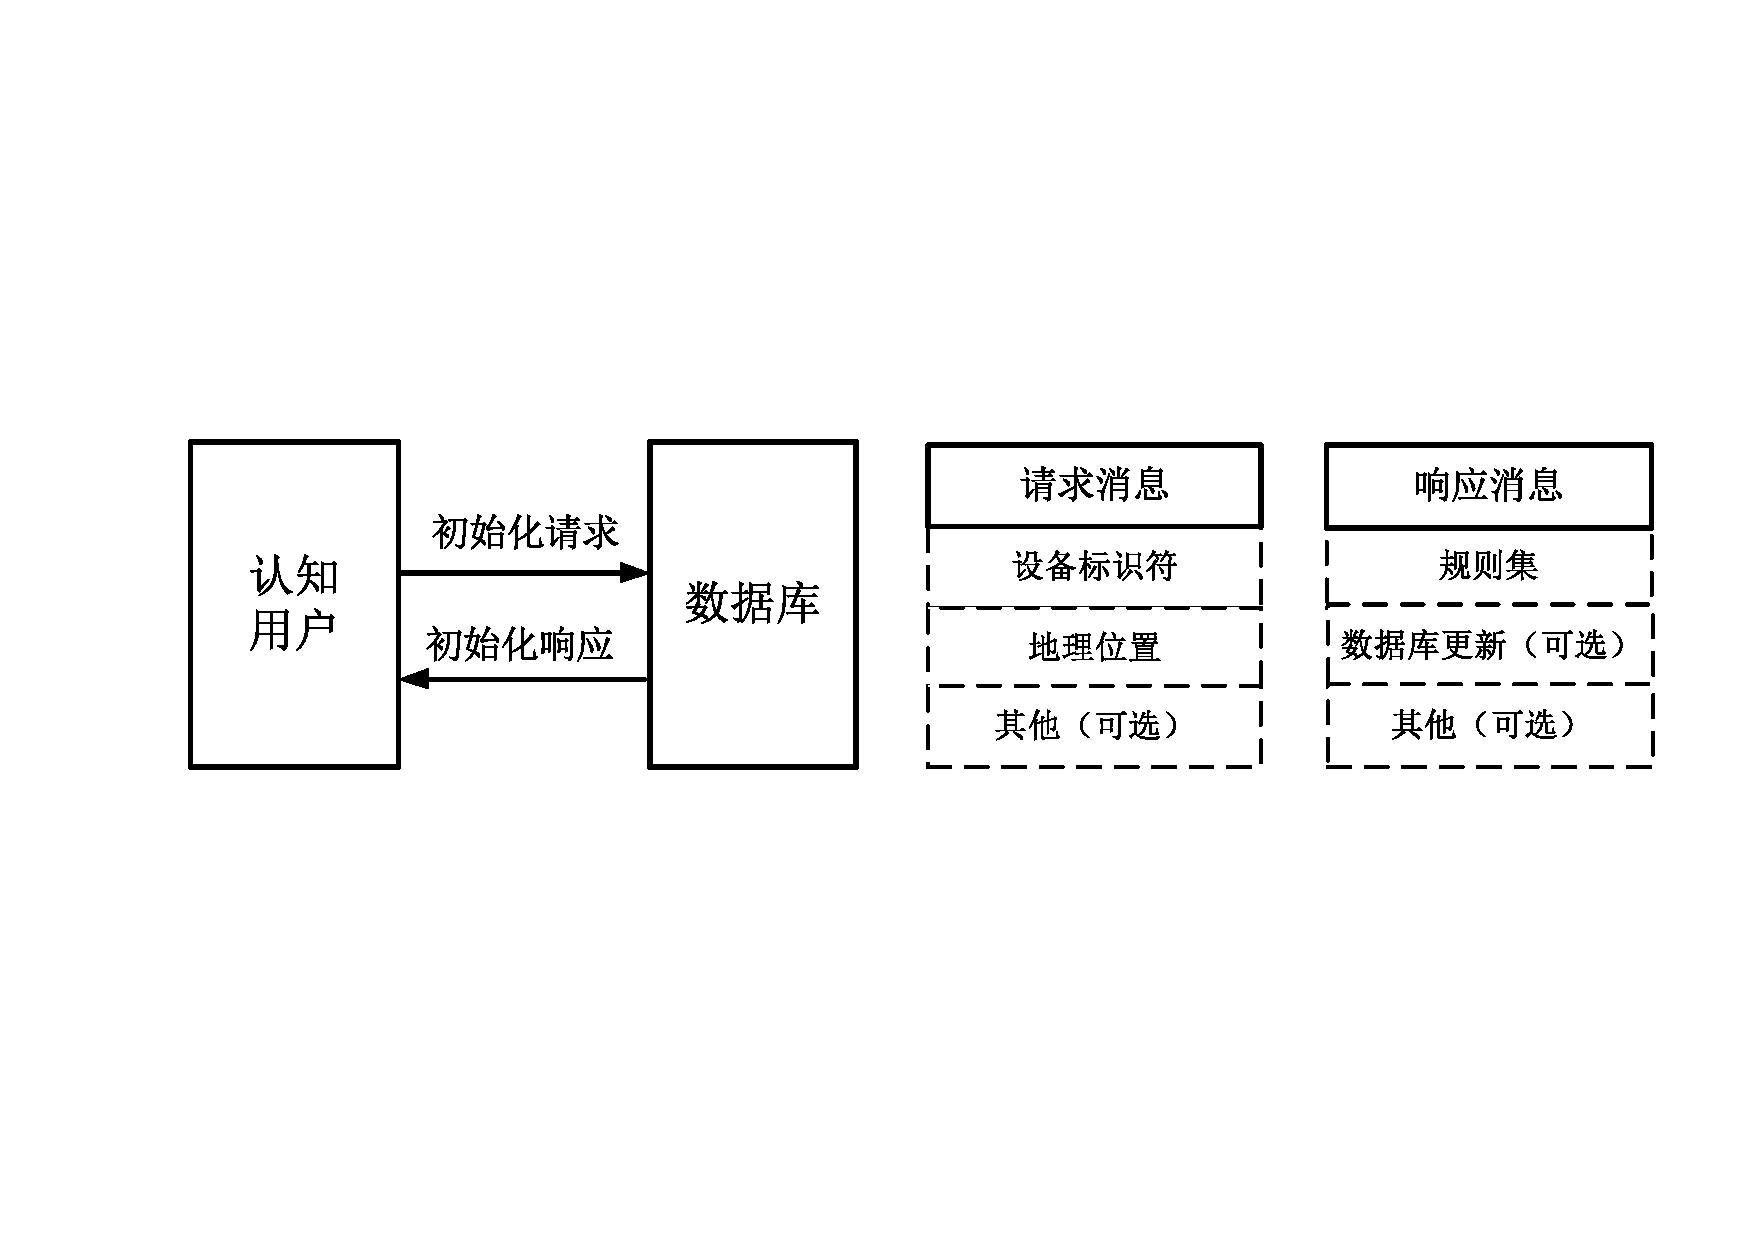
\includegraphics[width=0.8\textwidth]{figures/chap3/standard/initialization}\bicaption[fig:initialization]{用户初始化过程}{用户初始化过程}{Fig}{Process of Initialization}
\end{figure}

设备标识符是用户身份的唯一标识,规则集是指数据库管辖范围内约定的通信规则。数据库更新字段用于在数据库更改URI时通知认知用户进行相应更改。

\item 设备注册:

有些规则集要求认知用户向数据库发送注册信息以设定某些操作参数,例如FCC规定固定用户必须将其设备所有者和操作者以及设备标识符、地理位置、天线高度等信息上报给数据库。数据库可以要求认知用户以独立的请求方式进行注册,也可以允许认知用户将注册消息作为可用频谱查询消息的子集发送给数据库。用户注册过程如图\ref{fig:registration}所示。

\begin{figure}[!htp]\label{fig:registration}
  \centering
  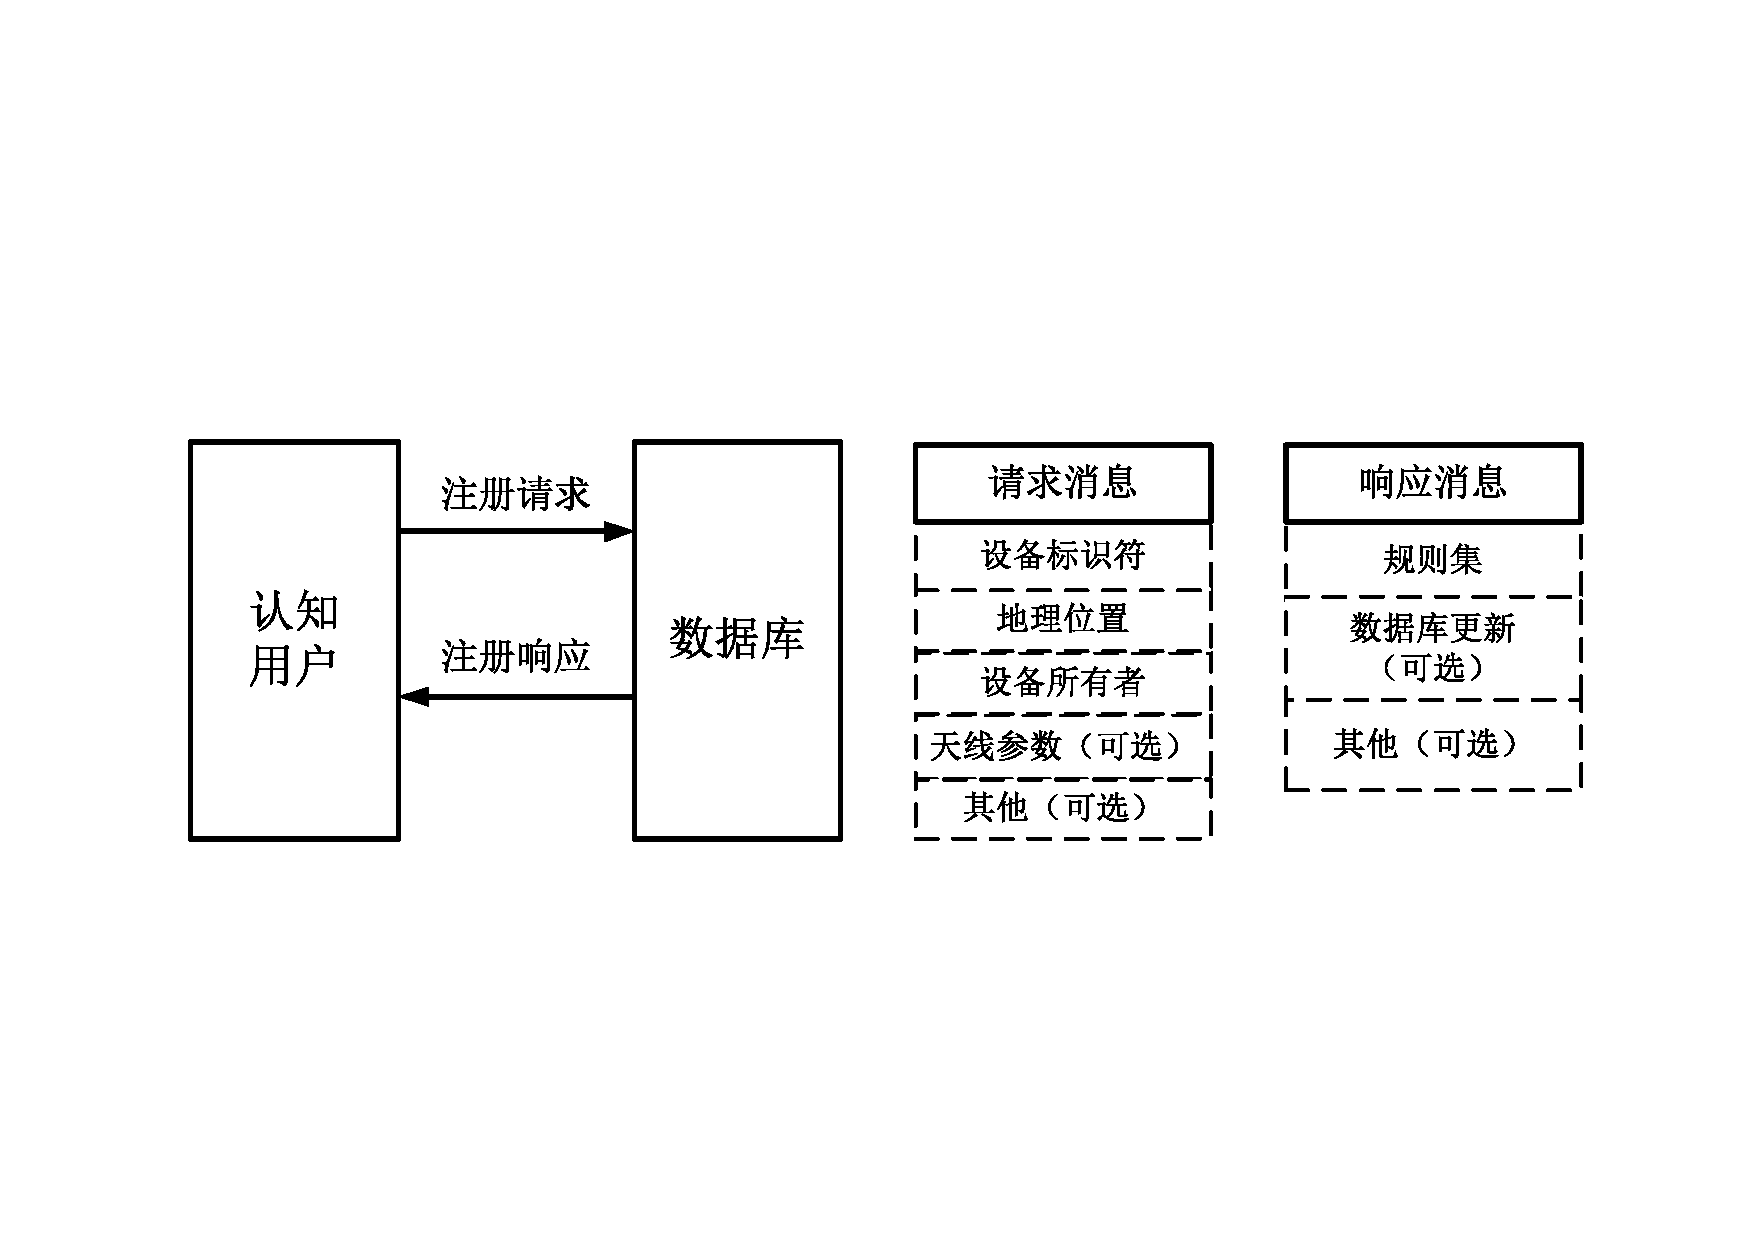
\includegraphics[width=0.8\textwidth]{figures/chap3/standard/registration}\bicaption[fig:registration]{用户注册过程}{用户注册过程}{Fig}{Process of Registration}
\end{figure}

设备所有者信息包含所有者的唯一身份标识。天线参数主要包括天线高度、天线类型、天线方向、天线辐射辐射类型、天线增益以及天线极化方式等信息。

\item 可用频谱查询及通知:

为从数据库获得可用频谱信息,认知用户发送查询消息,根据其地理位置和必须的参数请求可用频谱。数据库根据请求消息中的地理位置将该位置的可用频谱信息告知认知用户。认知用户在可用的频谱列表中进行选择并可以将频谱使用信息上报给数据库。可用频谱查询及通知过程如图\ref{fig:query}所示。

\begin{figure}[!htp]\label{fig:query}
  \centering
  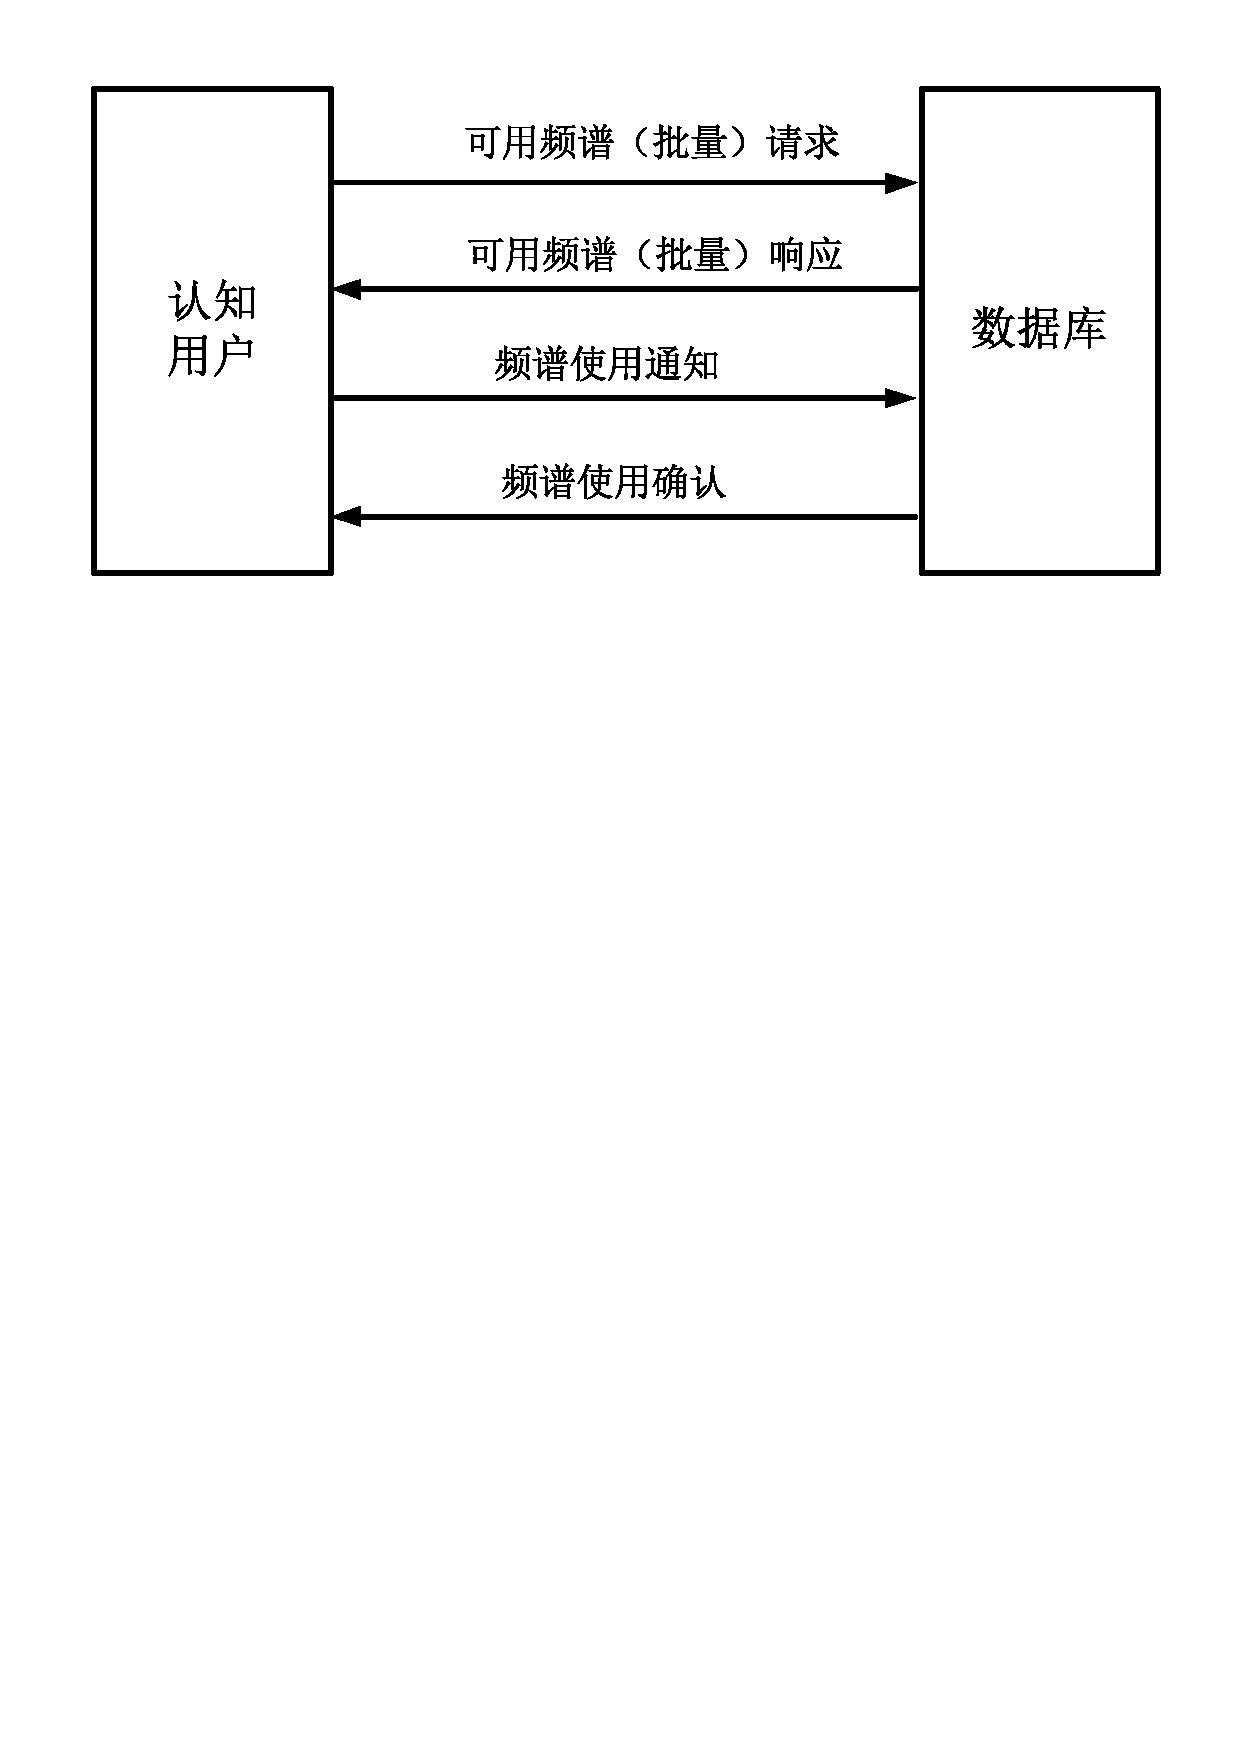
\includegraphics[width=0.6\textwidth]{figures/chap3/standard/query}\bicaption[fig:query]{可用频谱查询过程}{可用频谱查询过程}{Fig}{Process of Availability Spectrum Query}
\end{figure}

其中查询及响应内容如图\ref{fig:query-1}所示。

\begin{figure}[!htp]\label{fig:query-1}
  \centering
  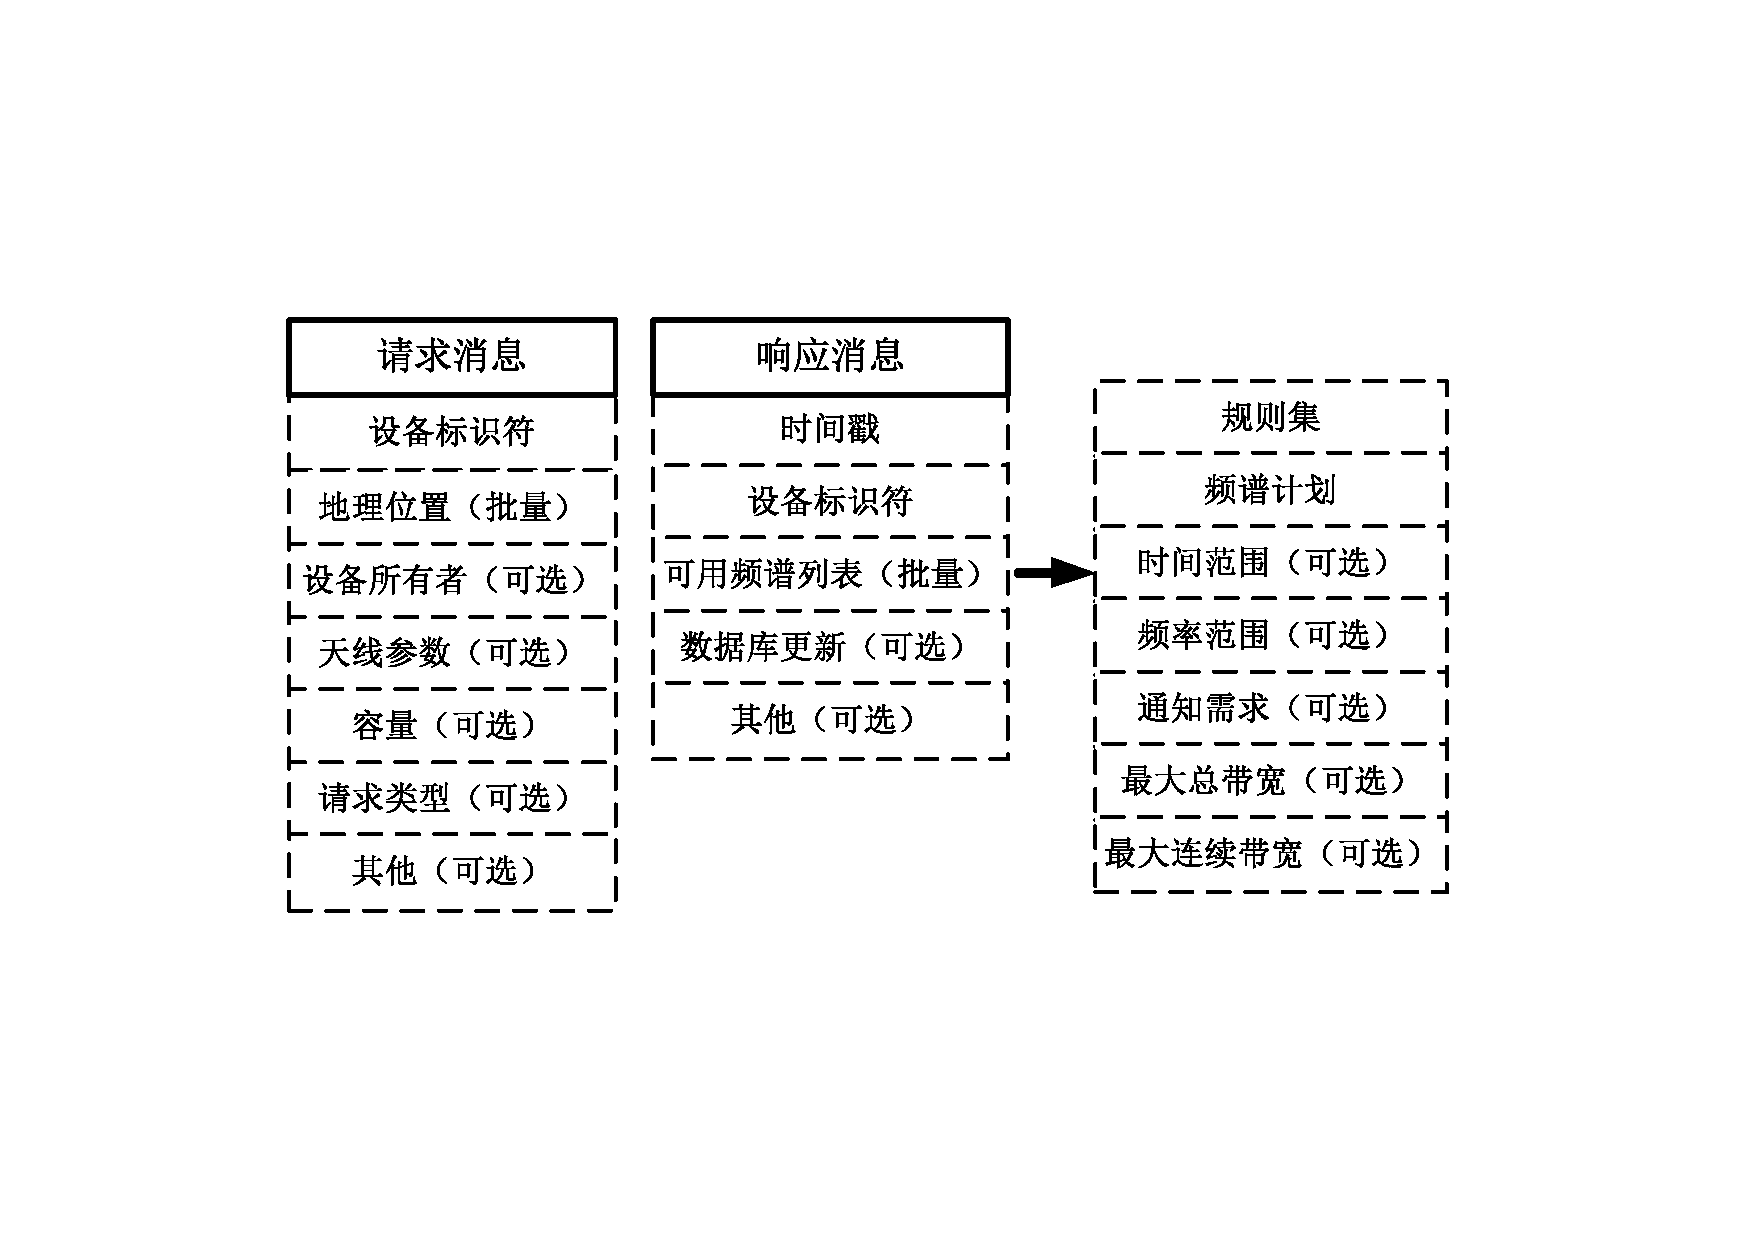
\includegraphics[width=0.65\textwidth]{figures/chap3/standard/query-1}\bicaption[fig:query-1]{频谱查询消息内容}{频谱查询消息内容}{Fig}{Contents of Spectrum Query Message}
\end{figure}

在批量查询的情况下,查询消息中可以包含多个地理位置,即同时请求这些位置上的可用频谱信息。容量字段可以使认知用户根据自身设备的容量指定请求的频段。请求类型字段使得认知用户可以声明一些其他的请求。

频谱使用通知及响应内容如图\ref{fig:query-2}所示。

\begin{figure}[!htp]\label{fig:query-2}
  \centering
  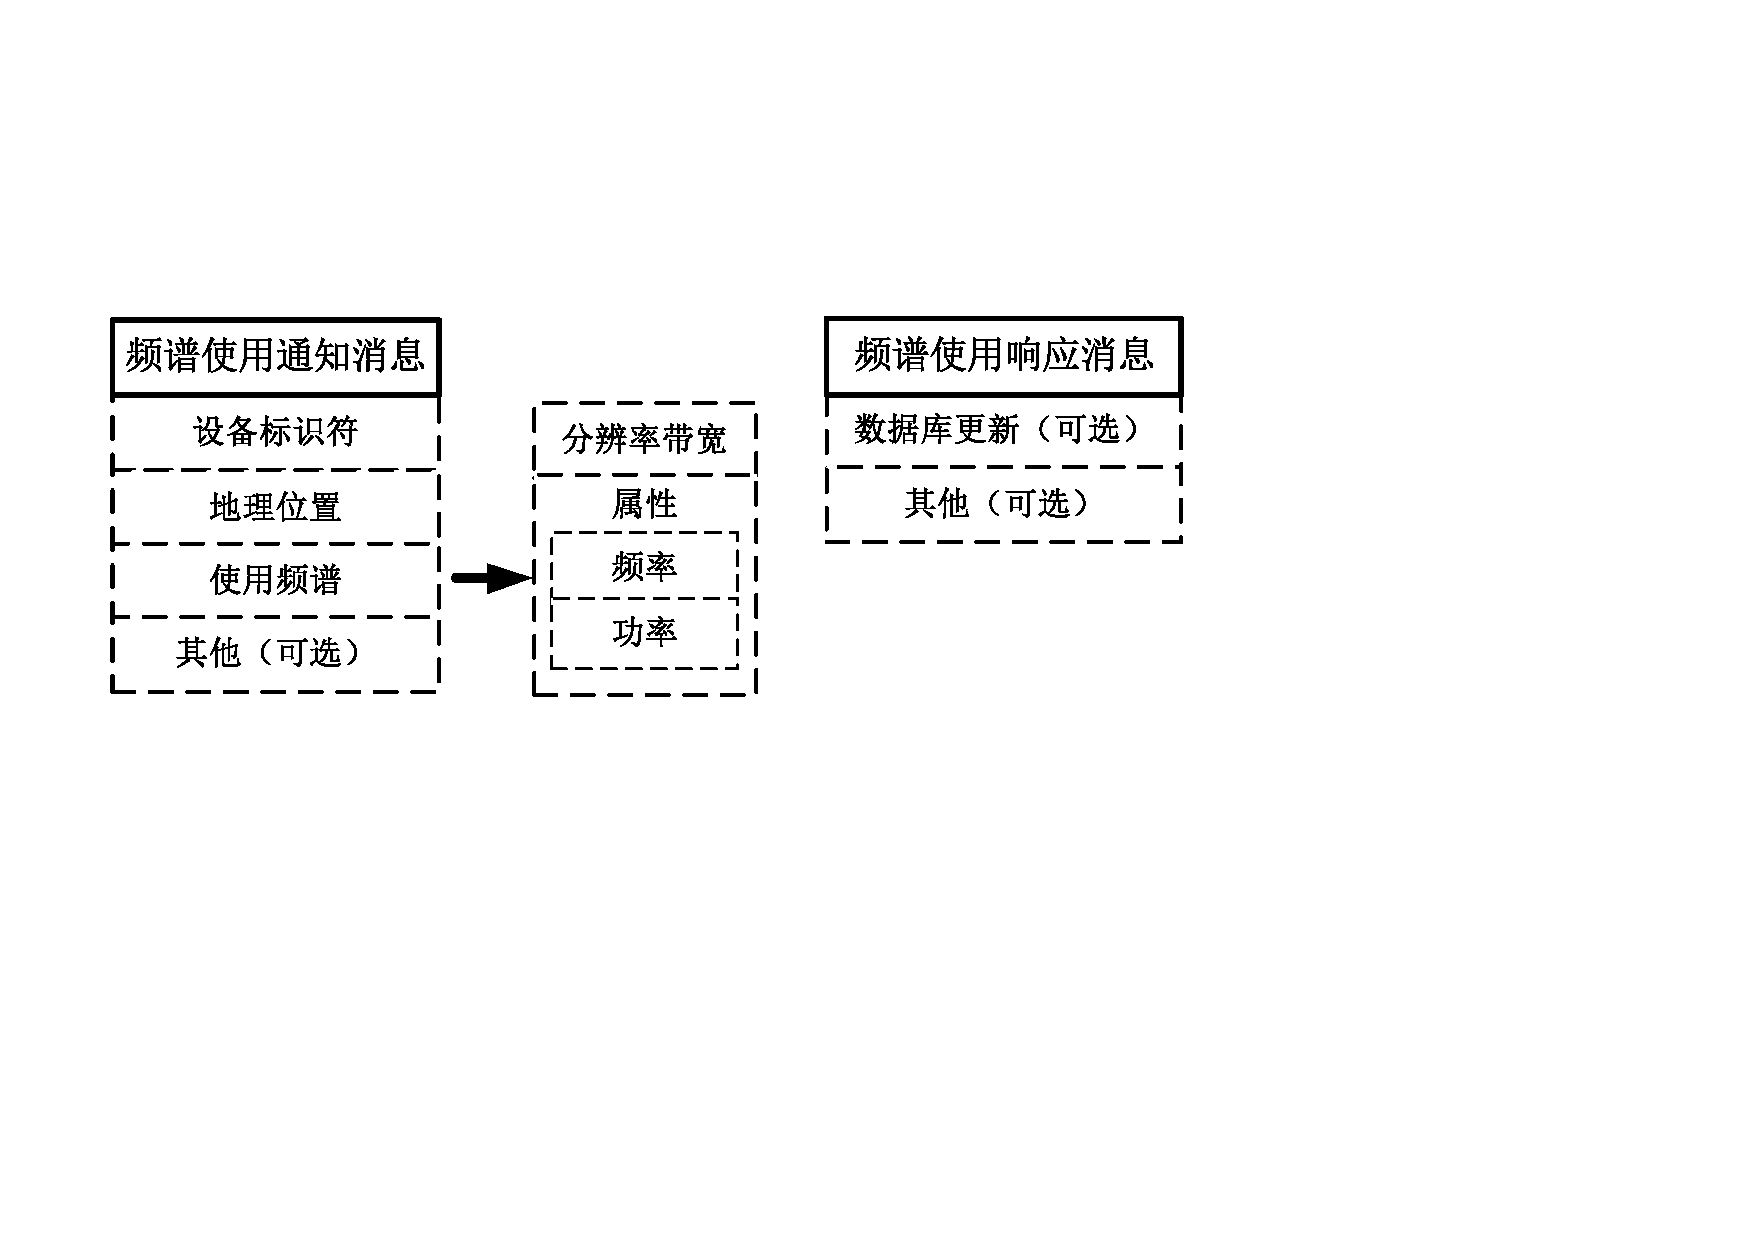
\includegraphics[width=0.65\textwidth]{figures/chap3/standard/query-2}\bicaption[fig:query-2]{频谱通知消息内容}{频谱通知消息内容}{Fig}{Contents of Spectrum Notification}
\end{figure}

频谱使用通知消息是可选功能,但若规则集采用此项功能,则认知用户必须将其使用的频谱和相应传输功率通报给数据库。

\end{enumerate}



HTTPS绑定:PAWS要求使用安全传输层协议(Transport Layer Security,TLS)作为底层的传输机制。TLS提供了认知用户和数据库之间传输消息的完整性和保密性。认知用户必须执行服务器认证,服务器也可以要求用户执行终端设备认证。
PAWS协议中的请求消息应该包含在HTTP POST请求消息中,响应消息应该包含在HTTP响应消息中。



安全方面的考虑:
在PAWS协议的框架下,认知用户和数据库面临如下安全风险:(1)精确度:认知用户收到不准确的可用频谱信息;(2)隐私:未授权者截获通信数据。为规避上述风险,PAWS需要依赖如下措施:

\begin{enumerate}
\item 认知用户必须确定合适的数据库用于查询。
\item 认知用户必须正确连接到合适的数据库。
\item PAWS消息需要保证不被篡改。
\item PAWS消息必须加密。
\end{enumerate}

PAWS允许通过静态指定安全的数据库来保证能够寻找到合适的数据库,采用TLS协议可以规避其他传输层以下的安全风险。此外,为避免精确度造成的风险,数据库需要具备准确计算可用频谱资源的能力,但这不在PAWS协议的考虑范围内。



%%==================================================
%% chapter04.tex for SJTU Master Thesis
%% Encoding: UTF-8
%%==================================================

\chapter{数据库驱动认知无线电网络中的位置推断攻击与保护}
\label{chap:fixed}

本章主要论述在数据库驱动认知无线电网络中固定用户所面临的位置隐私泄露以及相应的隐私保护方法。本章及后续部分所参考的依据主要为IETF发布的Internet草案和FCC公布的相关规定。

\section{系统模型}\label{sec:model}

在数据库驱动认知无线电网络中,我们假设数据库$DB$服务的区域$R$可以划分为$n \times n$个小区域,表示为$c_{ij}$,其中$i,j$分别是行索引和列索引。为方便描述,我们假定每个区域内的频谱可用信息相对稳定。网络中共有$C$个频道$ch_{1},...,ch_{k},...,ch_{C}$和$C$个主用户$PU_{1},...,PU_{i},...,PU_{C}$,即每个频道上有且只有一个主用户。可用频谱信息表示为$((ch_{1},P_{1},t_{1}),(ch_{2},P_{2},t_{2}),...,(ch_{k},P_{k},t_{k}))$。这里$ch_{i}$表示频道,$P_{i}$为$ch_{i}$上的允许发射功率,$t_{i}$为$ch_{i}$的预计可用时间。本文仅考虑可用频谱查询过程中的频道和功率信息,可用时间信息暂不列入考虑范围,因此可简化表示为$((ch_{1},P_{1}),(ch_{2},P_{2}),...,(ch_{k},P_{k}))$。可用频谱信息是数据库根据网络和地理环境进行计算的,主要考虑因素包括主用户的位置和发射参数、认知用户的发射参数、以及相关地理环境信息。认知用户允许发射功率$P_{i}$分为若干等级,由数据库根据最大传输功率(Maximum Transmission Power, MTP)函数进行计算得到。为方便起见,我们假设MTP函数只跟相对距离有关,即某个位置的认知用户在$ch_{i}$上所允许的最大发射功率$P_{i}$由该位置与$PU_{i}$所在位置的物理距离决定。公式\ref{eq:mtp}为MTP函数的一个示例。当距离小于$d_{0}$时,认知用户不允许发射以避免对主用户造成干扰;当距离超出范围$d_{n}$时,认知用户所允许的最大发射功率被定义为$P_{max}$,其具体值由FCC等机构规定,一般为100mW;当距离处于$d_{0}$和$d_{n}$之间时,认知用户允许以受限制的功率($<P_{max}$)工作。

\begin{equation}\label{eq:mtp}
P=\left\{
\begin{aligned}
&0  \quad when \ d(X)<d_{0} \\
&P_{1} \quad when \ d_{0} < d(X) \leq d_{1} \\
&... \\
&P_{max} \quad when \ d(X) > d_{n}
\end{aligned}
\right.
\end{equation}

基于IETF对数据库驱动认知无线电网络中可用频谱查询过程的规定,我们认为可用频谱查询的过程如下:

(1)请求:认知用户$SU_{i}$通过定位模块获取自身地理位置并向数据库发送请求消息,消息格式为$Que=(ID_{i},loc_{i})$。$ID_{i}$是$SU_{i}$的设备标识符及唯一身份标识,$loc_{i}$是$SU_{i}$的地理位置。我们假定认知用户可以同时查询其附近多个地理位置的可用频谱信息。

(2)响应:数据库在收到查询消息并提取地理位置信息后,计算该位置可用频谱信息并向认知用户发送响应消息,消息格式为$Res=(c_{ij},ch_{i},P_{i})$。

(3)通知:尽管在IETF制定的草案中,这个步骤是可选的,但是数据库作为网络中的服务提供者和管理者,需要根据认知用户的接入情况计算可用频谱信息,因此我们假定认知用户需要上报使用的频道信息,消息格式为$Not=(ID_{i},ch_{i},P_{i})$。


\section{针对静止用户的位置推断攻击}\label{sec:attack-fixed}

根据上述可用频谱查询过程,$DB$可以直接获得$SU$的地理位置信息。文献\cite{gao2013location}提出了一种基于私有信息提取的盲化查询机制,使得认知用户的地理位置信息在查询过程中对数据库是不可见的。事实上,即便在不直接获取认知用户位置的前提下,我们仍然可以根据可用频谱查询过程中的通信内容与用户位置的相关性对用户位置进行推测。因此,本文提出的攻击方法假设数据库无法直接获得认知用户的地理位置。本节工作主要考虑网络中主用户和认知用户都静止的情况。

如上所述,在可用频谱查询过程中,$DB$向$SU$提供某些地理位置上的可用频谱信息,包括可用的频道$ch_{i}$和该频道允许的最大发射功率$P_{i}$。由于$ch_{i}$所允许的发射功率$P_{i}$主要由认知用户与该频道主用户$PU_{i}$之间的距离所决定,因此认知用户可以根据$P_{i}$对它与$PU_{i}$之间的距离进行估算从而经过若干轮查询后能够逐渐确定$PU_{i}$的位置。认知用户在确定使用的频道$ch_{i}$后,需要向$DB$上报$ch_{i}$以及$P_{i}$。类似地,$DB$可以对认知用户与$PU_{i}$之间的相对距离进行估算,进而在经过若干轮查询后逐渐确定认知用户的位置。我们发现在频谱查询过程中,无论响应消息还是通知消息,都可以表示为一个可用频谱信息单元$(ch_{i},P_{i})$,而每个单元都含有一定的相对距离信息,从而可以根据MTP函数将$(ch_{i},P_{i})$转换为一个区域覆盖范围,进而我们基于网络中可能出现的两种隐私泄露情况提出如下相应的两种位置推断攻击。

\subsection{基于受限功率的位置推断攻击}
$DB$向认知用户提供的可用频谱信息可以简化为若干个可用频谱单元:$((ch_{1},P_{1}),...,(ch_{i},P_{i}),...,(ch_{C},P_{C})$。最大传输功率$P_{i}$被分为若干离散的功率等级,从而能够提高网络的服务效率。在理想的情况下,我们可以假设每个功率等级的覆盖范围为圆形区域或圆环型区域。如图\ref{fig:limited}所示,若认知用户$SU_{i}$收到关于$ch_{i}$的可用频谱信息单元$(ch_{i},P_{i})$,则它可以认为自己与主用户$PU_{i}$之间的距离大致在$d_{1} \sim d_{2}$之间,即$PU_{i}$有较大的概率处于左侧图中阴影环形区域内。同理,若$SU_{i}$上报的使用频道的最大发射功率为$P_{i}$,则$DB$可以认定$SU_{i}$有较高的概率处于右图中阴影区域内。

\begin{figure}[!htp]\label{fig:limited}
  \centering
  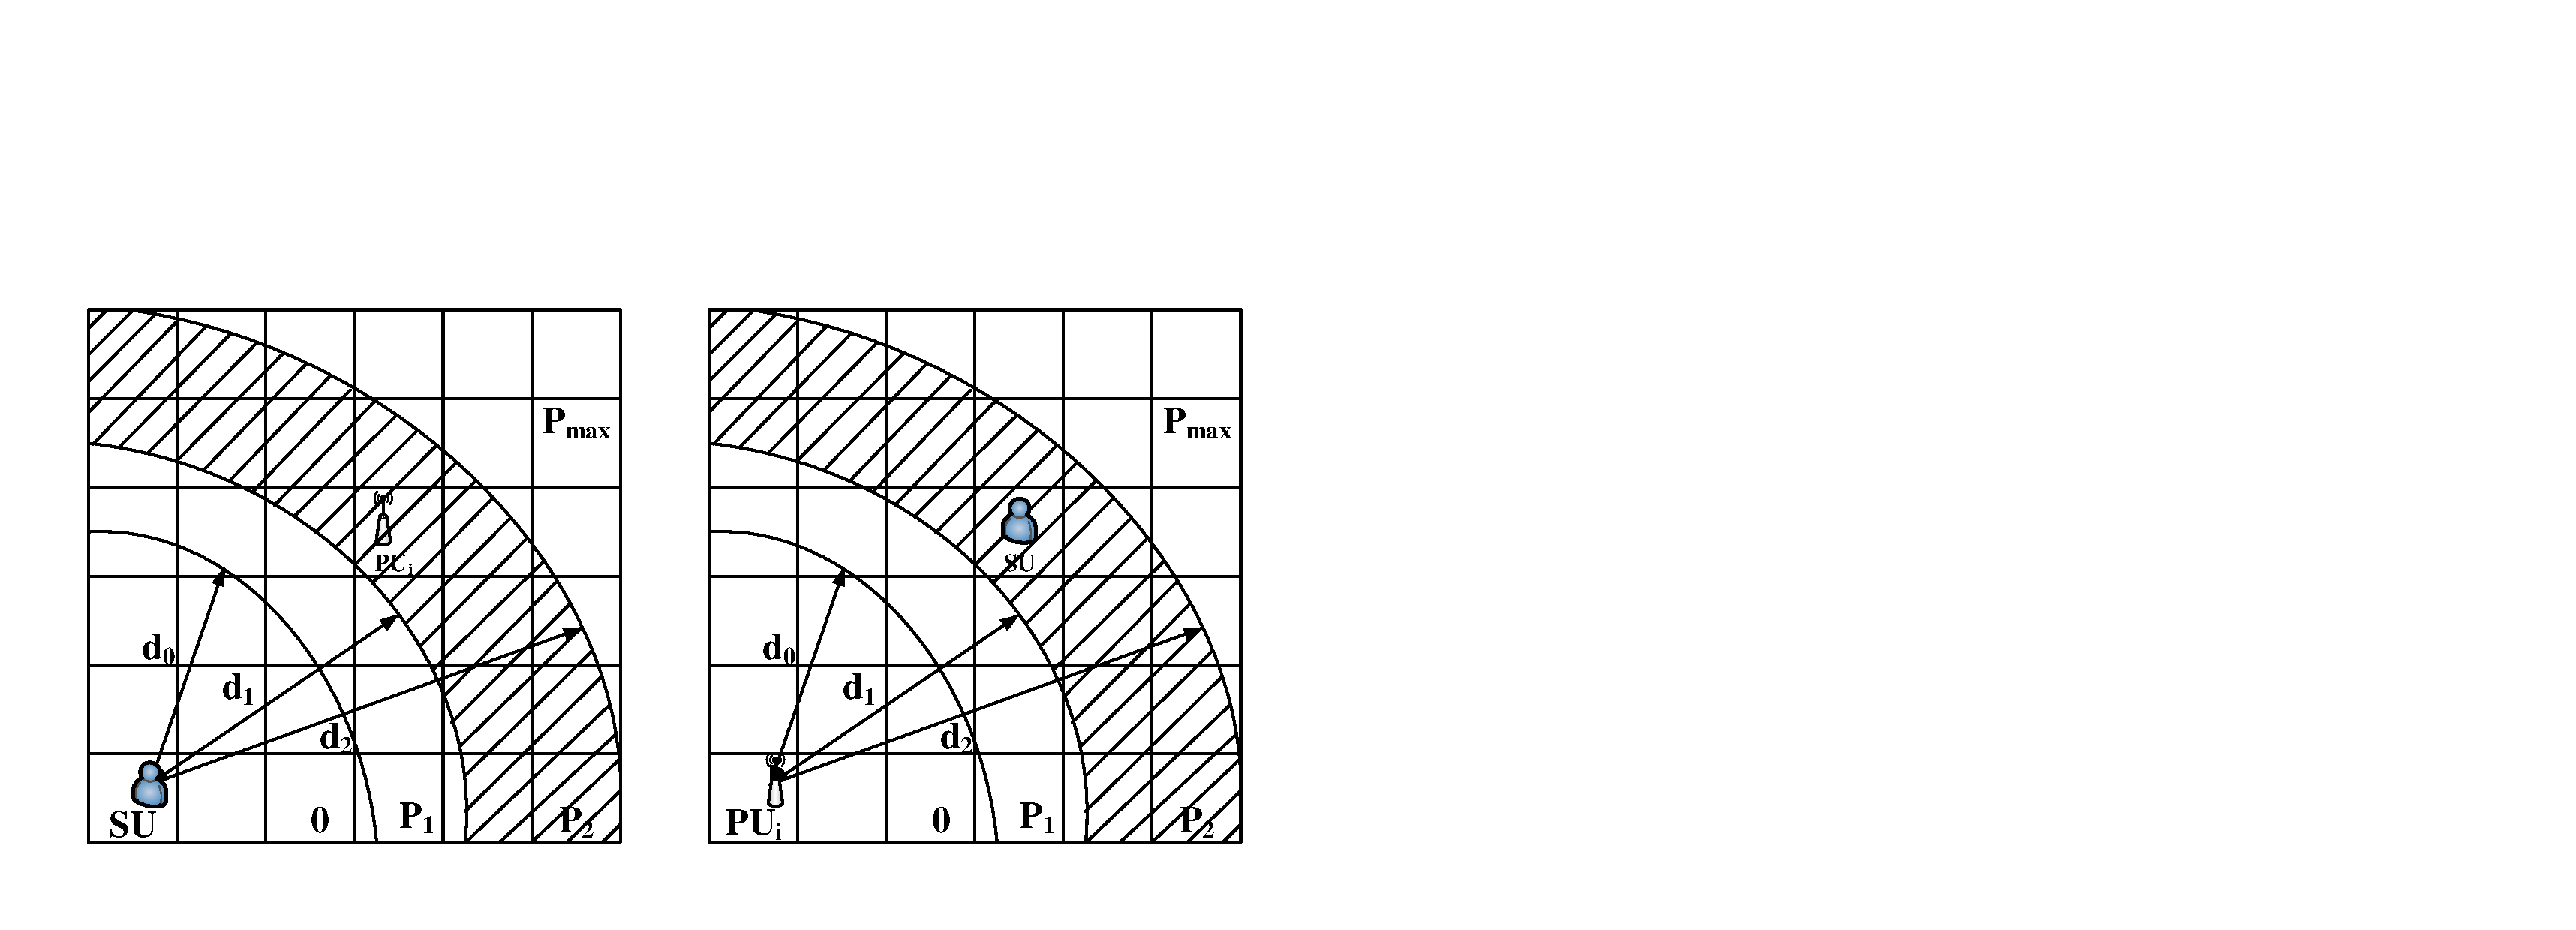
\includegraphics[width=0.8\textwidth]{figures/chap4/limited}\bicaption[fig:attack:limited]{基于受限功率的位置推断攻击示意图}{基于受限功率的位置推断攻击示意图}{Fig}{Illustration of Attack Based on Limited Power}
\end{figure}

若$SU_{i}$持续选择功率受限的频道,那么随着时间的推移,攻击者可以将每一次的覆盖范围进行取交集操作从而实现对静止的$SU_{i}$的比较精确的位置推断。

\subsection{基于频道切换的位置推断攻击}

为确保认知用户在使用频谱过程中不会对主用户产生任何干扰,当主用户在线时,认知用户不允许在主用户的保护范围内以相同的频道发射功率。主用户的保护区域一般是一个以主用户为圆心的圆形区域,假设保护区域半径为$d_{0}$。当主用户$PU_{i}$在线时,这个区域内不允许任何认知用户在$ch_{i}$工作。因此可能出现的一种情况是,$PU_{i}$不在线,某个认知用户$SU_{i}$处于主用户$PU_{i}$的保护范围内且正在使用$ch_{i}$,一旦$PU_{i}$上线,则$DB$会通知$SU_{i}$立即腾出$ch_{i}$。基于这个切换事件,$SU_{i}$立即得知,$PU_{i}$有很大概率处于以$SU_{i}$所在位置为圆心,以$d_{0}$为半径的圆形区域内。同理,若$DB$计算出某个$SU_{i}$不允许在$ch_{i}$上发射,则$DB$可以认为$SU_{i}$有较大概率处于$PU_{i}$的保护范围内。基于频道切换的位置推断攻击如图\ref{fig:switch}所示。

\begin{figure}[!htp]\label{fig:switch}
  \centering
  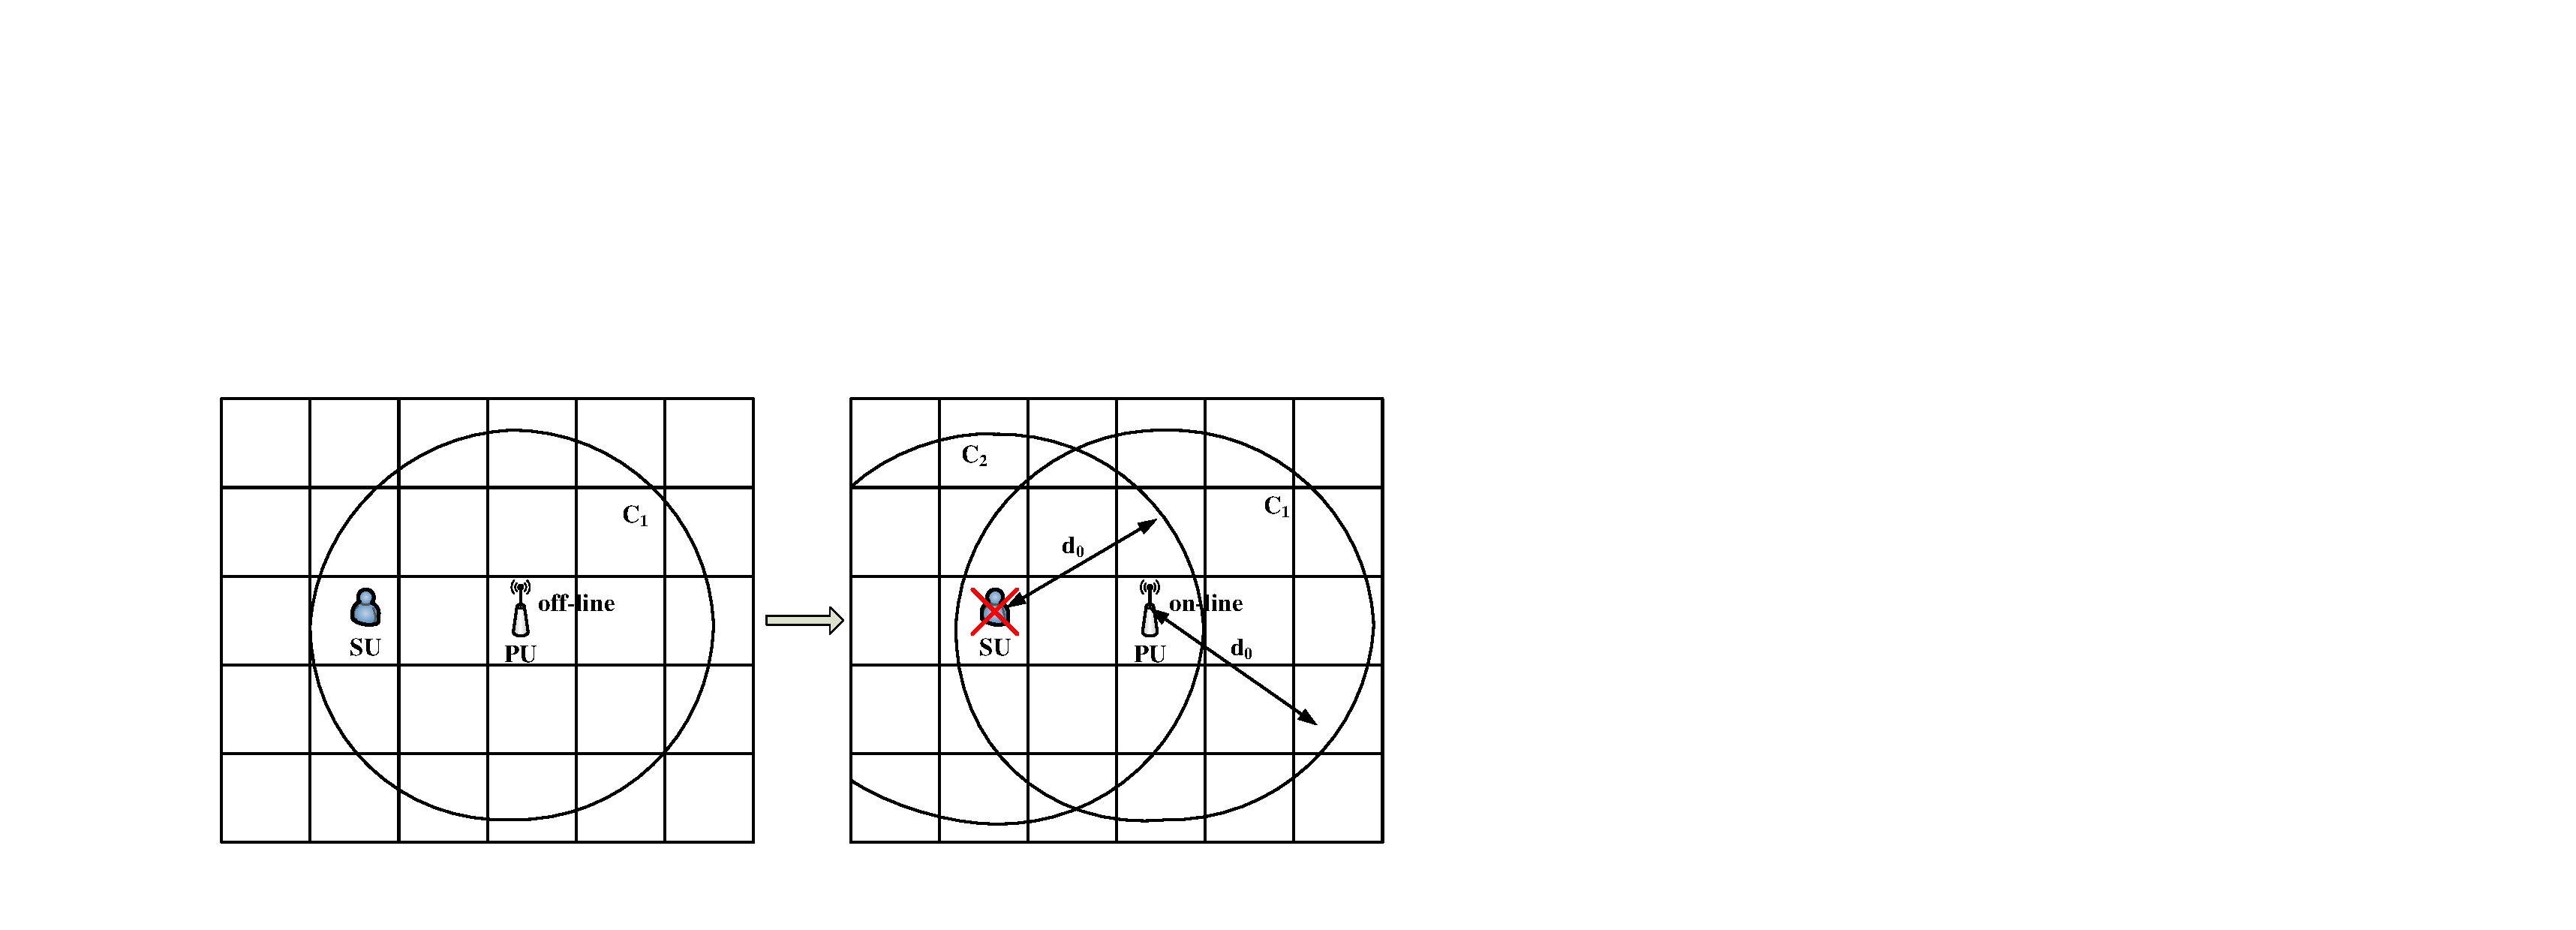
\includegraphics[width=0.8\textwidth]{figures/chap4/switch}\bicaption[fig:switch]{基于频道切换的位置推断攻击示意图}{基于频道切换的位置推断攻击示意图}{Fig}{Illustration of Attack Based on Channel Switch}
\end{figure}

由于主用户的保护范围为圆形区域,覆盖范围相比其他情况要小,因此频道切换事件会更加严重地泄露认知用户和主用户的位置隐私。

\subsection{统一的位置推断攻击算法}\label{alg-attack}

根据如上分析,在数据库驱动认知无线电网络中,认知用户和数据库在位置推断攻击的层面上是对立的。一方面认知用户可以根据数据库提供的可用频谱信息危害网络中主用户的位置隐私;另一方面数据库可以根据提交的频道信息危害认知用户的位置隐私。因此,我们认为在可用频谱查询过程中主用户和认知用户的隐私同时存在被对方攻击的风险。根据可用频谱查询过程中认知用户和数据库之间传输的可用频谱信息单元$(ch_{i},P_{i})$,我们提出了一种一般化的攻击方案。算法\ref{alg:fixed}是该攻击方法的伪代码描述。

\begin{lstlisting}[language={C}, caption={统一的位置推断攻击算法}]
输入:攻击者的位置$loc$,频谱单元序列$((ch_{1},P_{1}),...,(ch_{i},P_{i}),...,(ch_{C},P_{C})$;攻击者先验知识$R'$。
输出:目标的可能位置集$L$
初始化:$L=\phi$;  $\delta$;  $n \times n$概率矩阵$PR$,$pr_{ij} \in PR$
for $0 \leq i \leq n$ and $0 \leq j \leq n$
    if $c_{ij} \in R'$
        $pr_{ij}=\frac{1}{2}$
    else
        $pr_{ij}=0$
for each ($ch_{i},P_{i}$)
    if 功率受限或频道切换事件发生
        M=Cov($ch_{i},P_{i}$) 
            for each $c_{ij} \in Cov(ch_{i},P_{i})$
                $pr_{ij}=\frac{pr_{ij}}{1-\frac{1}{|M|}(1-pr_{ij})}$ 
                if $pr_{ij} \geq \delta$
    $L = L \cup c_{ij}$
    return $L$
Cov($ch_{i},P_{i}$):
    $d_{min},d_{max}$ = $P_{i}$对应距离范围的边界值
    X = $\phi$
    for $c_{ij} \in R'$
        if $d_{min} \leq distance(c_{ij},loc) \leq d_{max}$
            $X = X \cup c_{ij}$
    return X
\end{lstlisting}\label{alg:fixed}

在算法\ref{alg:fixed}中,攻击者可能具有对目标的先验知识,即目标的可能位置分布,这可以缩小对目标位置的推测范围。$M$代表频谱信息单元$(ch_{i},P_{i})$对应的覆盖范围,$|M|$是范围内包含的小区域数量。我们根据公式\ref{eq:bayes}所述的贝叶斯规则\cite{bahrak2013ex},在每一轮迭代中将可能作为候选的区域对应的概率值逐渐增加,直到超过预先设定的阈值$\delta$,则认定该区域可能是攻击目标所处的位置。我们将在本章最后对攻击效果进行验证。
\begin{equation}\label{eq:bayes}
pr_{ij}=\frac{pr_{ij}}{1-\frac{1}{|M|}(1-pr_{ij})}
\end{equation}

\section{针对位置推断攻击的解决方案}

为解决数据库驱动认知无线电网络中静止用户的隐私泄露问题,我们必须同时考虑两个方面的问题:服务质量和隐私保护。在数据库驱动认知无线电网络环境下,服务质量即为频谱效益。对认知用户来讲,它是网络服务的使用者,主要关注自身所能够获得的频谱质量;对数据库来讲,它是整个网络的服务提供者,需要为全局尽量提供较好的频谱质量。一般来讲,无论对于服务提供者还是服务使用者,服务质量和隐私保护效率都是一对矛盾的双方。例如在传统的LBS中,用户如果想获得更好更准确的周边信息服务,那就必然要向服务提供者提交更加精确的位置,因而也会导致位置隐私泄露更加严重。任何隐私保护的方案一定是以牺牲某方面的服务性能为代价的。在本节,我们提出一个频谱查询过程中的隐私保护框架,使得认知用户和数据库可以根据自身需求,在满足一定服务质量的前提下,最好地保护自身隐私。为方便描述,我们必须首先对服务质量和隐私给出一个量化的定义。

\subsection{频谱效益和隐私的度量}

\subsubsection{频谱效益的度量}

对于频谱效益,我们可以直观地采用无线信道容量作为其度量标准。信道容量是由通信链路上的信号与干扰噪声强度比来决定的(Signal to Interference and Noise Ratio, SINR),认知用户获得的通信链路的SINR可由公式\ref{eq:SINR}计算\cite{capacity}。

\begin{equation}\label{eq:SINR}
SINR  = \frac{P_{sec}/L_{sec}(r_{cell})}{N_{0}W_{0}+I_{P2S}+I_{S2S}}
\end{equation}

在公式\ref{eq:SINR}中,$P_{sec}$为认知用户的发射功率,$L_{sec}(r_{cell})$为小区域中认知用户发射接收链路的损耗。$N_{0}$为认知用户接收机的噪声功率谱密度,$W_{0}$是认知用户的信道带宽,$I_{P2S}$是主用户对认知用户的干扰,$I_{S2S}$是认知用户之间的干扰。

在小区域$c$内的频道$ch_{i}$上获得的平均信道容量可以由公式\ref{eq:capacity}表示\cite{capacity}。
\begin{equation}\label{eq:capacity}
Cap_{c}^{i}  = W_{0} \int_{c} \frac{log_{2}(1+SINR(l))}{c}dl
\end{equation}

为简化实际模型的表示,我们假设信道容量在小区域$c$范围内相对稳定,因此可将认知用户在$ch_{i}$上获得的信道容量重写为:
\begin{equation}\label{eq:capacity-revised}
Cap_{c}^{i}  = W_{0} log_{2}(1+SINR^{i})
\end{equation}

对于网络中的认知用户,他们只关心所使用频道的容量而与数据库提供的其他可选频道无关,因此认知用户的频谱效益可以表示为公式\ref{eq:util-su}。
\begin{equation}\label{eq:util-su}
Util_{SU}=\frac{1}{|CH|}\sum\limits_{ch_{i} \in CH} Cap_{c}^{i}
\end{equation}
式中$CH$为认知用户使用过的频道列表,$|CH|$为集合元素个数,上式的意义为认知用户历史上使用过的频谱服务总量。


对于数据库来说,他关心为每个用户所提供的总的服务能力,因此提供的可选择频道越多,频道的容量越大,则服务质量越好,于是我们使用公式\ref{eq:util-db}来表示数据库针对某个认知用户的频谱效益:
\begin{equation}\label{eq:util-db}
Util_{DB}=\frac{1}{|CH_{A}|} \sum\limits_{ch_{i} \in CH_{A}} Cap_{c}^{i}
\end{equation}

$CH_{A}$是数据库为认知用户提供的可用频道的集合,$|CH_{A}|$为集合元素个数。公式\ref{eq:util-db}的意义是数据库为某个认知用户提供的平均信道容量。

\subsubsection{隐私的度量}

对位置隐私进行度量的常用方式是采用位置的不确定性。假设可能的位置集为$L=(l_{1},l_{2},...,l_{n})$,在这些位置上的概率分布为$(p_{1},p_{2},...,p_{n}),\sum\limits_{i=1}^{n} p_{i} = 1$。根据熵公式,位置不确定性可表示为公式\ref{eq:uncertainty}:
\begin{equation}\label{eq:uncertainty}
UnC=-\sum\limits_{i=1}^{n}p_{i}log p_{i}
\end{equation}

使用不确定性作为隐私度量方式的问题是,它无法准确地描述攻击者对位置的估计误差。此外,基于我们提出的攻击算法,攻击目标处于可能位置集合$L$中所有位置的概率是相等的,都是$1/|L|$,其中$|L|$是集合$L$中元素个数。因此,我们可采用平均误差距离作为隐私的度量方式。我们将\ref{alg-attack}中的攻击算法表示为条件概率密度函数$A(loc'|\cdot)$,$\cdot$为算法中的输入信息,$loc'$为攻击者推断出的位置。那么隐私可以表示为公式\ref{eq:privacy}。

\begin{equation}\label{eq:privacy}
Priv=\sum\limits_{loc' \in L} A(loc'|\cdot)d(loc,loc')
\end{equation}

其中函数$d()$是两个位置之间的欧氏距离,$loc$为攻击目标的真实地址,$loc'$为攻击者推断的地址。


\subsection{隐私保护的频谱查询方案}\label{subsec:privacy-preserving}

为减少可用频谱查询过程中的位置隐私泄露,我们提出一种改进的频谱查询方案如下:
\subsubsection{基于$k$-anonymity的请求}
认知用户同时查询包含$K_{Q} \times K_{Q}$个小区域的正方形区域$B$内的可用频谱信息。若考虑节省通信开销的问题,可以从$B$中随机挑选若干位置进行查询。认知用户可以将周边区域的可用频谱信息作为频道选择的参考。图\ref{fig:cloaking}为基于$k$-anonymity的请求示意图。

\begin{figure}[!htp]\label{fig:cloaking}
  \centering
  \includegraphics[width=0.8\textwidth]{figures/chap4/cloaking}\bicaption[fig:cloaking]{基于$k$-anonymity的可用频谱请求示意图}{基于$k$-anonymity的可用频谱请求示意图}{Fig}{Available Spectrum Query Based on $k$-anonymity}
\end{figure}

\subsubsection{基于$k$-anonymity的响应}
为弱化攻击者对主用户位置的推理攻击,我们采用文献\cite{bahrak2014protecting}中提出的基于$k$-anonymity的隐私保护方案,将网络中的主用户进行分组的办法来保护主用户的位置隐私。具体方法是将距离最近的主用户划分为若干个组,每一组有至少$K_{R}$个用户。我们认为每一个用户组是一个虚拟的主用户,其保护区域覆盖了内部所有主用户的保护区域。这样,数据库根据虚拟的主用户信息来计算可用频谱信息,在牺牲一些可用频谱资源的前提下,能够在一定程度上模糊主用户的真实位置,如图\ref{fig:anonymity}所示。

\begin{figure}[!htp]\label{fig:anonymity}
  \centering
  \includegraphics[width=0.8\textwidth]{figures/chap4/anonymity}\bicaption[fig:anonymity]{基于$k$-anonymity的可用频谱响应示意图}{基于$k$-anonymity的可用频谱响应示意图}{Fig}{Illustration of Available Spectrum Response Based on $k$-anonymity}
\end{figure}
在对主用户进行分组时,我们首先尽量选择最近的$K_{R}$个主用户分为一组,然后我们需要找到能够覆盖这$K_{R}$个位置的最小覆盖圆。假设最小覆盖圆的圆心为$X$,半径为$R_{X}$,则我们可以通过解决如下问题来找到$X$和$R_{X}$。

\begin{equation}
\min_{X} \max_{loc_{i}} {d(loc_{i},X)}
\end{equation}
其中,$loc_{i}$为主用户的地址,函数$d()$为两个点之间的欧氏距离。
然后我们可以将MTP函数修改为:
\begin{equation}\label{equation:mtp-altered}
P(loc)=\left\{
\begin{aligned}
&0  \quad when \ d(loc,X)<R_{X}+ d_{0} \\
&P_{1} \quad when \ R_{X}+d_{0} < d(loc,X) \leq R_{X}+d_{1} \\
&... \\
&P_{max} \quad when \ d(loc,X) > R_{X}+d_{n}
\end{aligned}
\right.
\end{equation}

这种基于$k$-anonymity的方法显然会增加主用户的位置隐私,因为它明显扩大了主用户的保护范围。同时,也必然会带来明显的频谱效益下降。此外,参数$K_{R}$的值对数据库的频谱效益和能够获得的隐私保护程度影响非常大,我们在后面讨论$K_{R}$的选择。

\subsubsection{改进的频道选择}

根据\ref{sec:attack-fixed}节分析的隐私泄露方式,若认知用户随机地选择满足要求的频道,则会遇到更多的功率受限和频道切换的情况,从而导致严重的隐私泄露。因此,在基于$k$-anonymity的可用频谱请求和响应的基础上,我们提出提出如下频谱选择方案。
(1)认知用户在所有查询的区域上都收到可用频谱信息单元$(ch_{i},P_{max})$,那么该认知用户有可能离主用户$PU_{i}$很远,也有可能意味着$PU_{i}$不在线。若是第二种情况而且认知用户恰好处于$PU_{i}$的保护范围内,那么很可能发生频道切换事件。因此,建议不使用这类频谱资源。
(2)认知用户在其所处的区域收到可用频谱信息单元$(ch_{i},P_{max})$,然而在其查询的其他区域关于$ch_{i}$的最大可用功率不全为$P_{max}$,那么说明$PU_{i}$一定在线,而且认知用户的位置距离主用户很远。这类可用频道既能允许较高的发射功率,又能较少的泄露位置隐私,因此较为推荐使用。
(3)认知用户在其所处的区域没有收到允许最大功率发射的可用频谱单元,那么他应该挑选允许发射功率最大的频道来使用,因为允许发射功率越大的频道对应的覆盖范围越大,而且信道质量越好。

\subsubsection{参数决定}
在上面提出的隐私保护的可用频谱查询框架中,为了在满足一定的频谱效益的前提下实现隐私保护的最大化,我们需要确定最合适的参数和选项。
对于数据库来讲,他应该力图在保证提供一定质量服务的前提下尽可能保护主用户隐私。因此根据前面的定义,我们可将数据库的频谱效益写为:

\begin{equation}
Util_{DB}=\frac{1}{K_{R}^{2}}\sum\limits_{c \in B} \sum\limits_{ch_{k} \in CH_{A}} Cap_{k}
\end{equation}

数据库的隐私保护程度可写为:

\begin{equation}
Pri_{PU}(loc,S(K_{Q},K_{R}))=\sum\limits_{loc' \in L} A(loc'|SAI(K_{Q},K_{R}))d(loc,loc')
\end{equation}

式中,$SAI(K_{Q},K_{R})$表示参数为$K_{Q},K_{R}$的情况下$DB$提供的可用频谱信息。若我们设定$\sigma_{DB}$为$DB$可忍受的最小频谱效益,则可以通过解决如下问题来得到最优的参数$K_{R}$。

\begin{equation}
\max_{K_{R}} Priv_{PU}(loc_{PU},SAI(K_{Q},K_{R})) 
\end{equation}

\begin{equation}
s.t. \quad Util_{DB} \geq \sigma_{DB}
\end{equation}

对于认知用户来讲,由于他们不知道网络中主用户的位置,所以无法自己计算隐私泄露程度,只能通过上面提出的方法优先选择合适的频道。但是在网络设计者的角度,我们可以给出类似的隐私定义并在具有网络全局知识的前提下,通过解决如下问题来计算能最大化认知用户隐私的最优频道:

\begin{equation}
\max_{ch_{i}} Priv_{SU}(loc_{SU},CH \cup ch_{i}) 
\end{equation}

\begin{equation}
s.t. \quad Util_{SU} \geq \sigma_{SU}
\end{equation}

式中$\sigma_{SU}$是认知用户所能容忍的最低的频谱效益。

\subsection{位置推断攻击与隐私保护的实验验证}
我们对文中提出的攻击方法和隐私保护方法的有效性进行了实验验证。从目前网络上公布的广播电视频段信号强度数据库来看,网络中的主用户即电视发射台一般集中部署,因此网络中大部分主用户几乎处于同一位置。然而未来的数据库驱动认知无线电网络一定不会局限于此类部署方式。因此,本文采用随机模拟的场景进行实验。

我们考虑数据库服务于一个$40km \times 40km$的区域,该区域划分为$400 \times 400$个$100m \times 100m$的正方形小区域。区域内有50个主用户、50个频道和随机分布的若干认知用户。假设最大传输功率量化为4个等级:0、1、2、3,其中等级0为不允许发射,等级3为$P_{max}$,其对应的覆盖范围如公式\ref{eq:coverage}所示。在数据库服务区域内,主用户随机切换在线/离线状态但不会太频繁。在不影响整体结果的条件下,度量频谱效益和隐私时,我们忽略了主用户对认知用户的干扰以及认知用户之间的干扰,直接采用功率等级来衡量信道容量。
\begin{equation}\label{eq:coverage}
P=\left\{
\begin{aligned}
&0 \quad when \ d < 8km \\
&1 \quad when \ 8km \leq d < 14km \\
&2 \quad when \ 14km \leq d < 25km \\
&3 \quad when \ d \geq 25km
\end{aligned}
\right.
\end{equation}
图\ref{fig:exp1-su}展示了对认知用户的攻击效果。可以看出,由于认知用户随机选择接入的频道,那么随着时间的增加,各种受限功率和频道切换事件发生的次数增加,于是导致其位置隐私逐渐泄露。一段时间之后,各种可能导致位置隐私泄露的事件都发生过,则认知用户可以最终被定位在一个较小的区域范围内,平均定位精度约25个小区域,范围大致相当于一个$500m \times 500m$的正方形区域。

\begin{figure}[!htp]
  \centering
  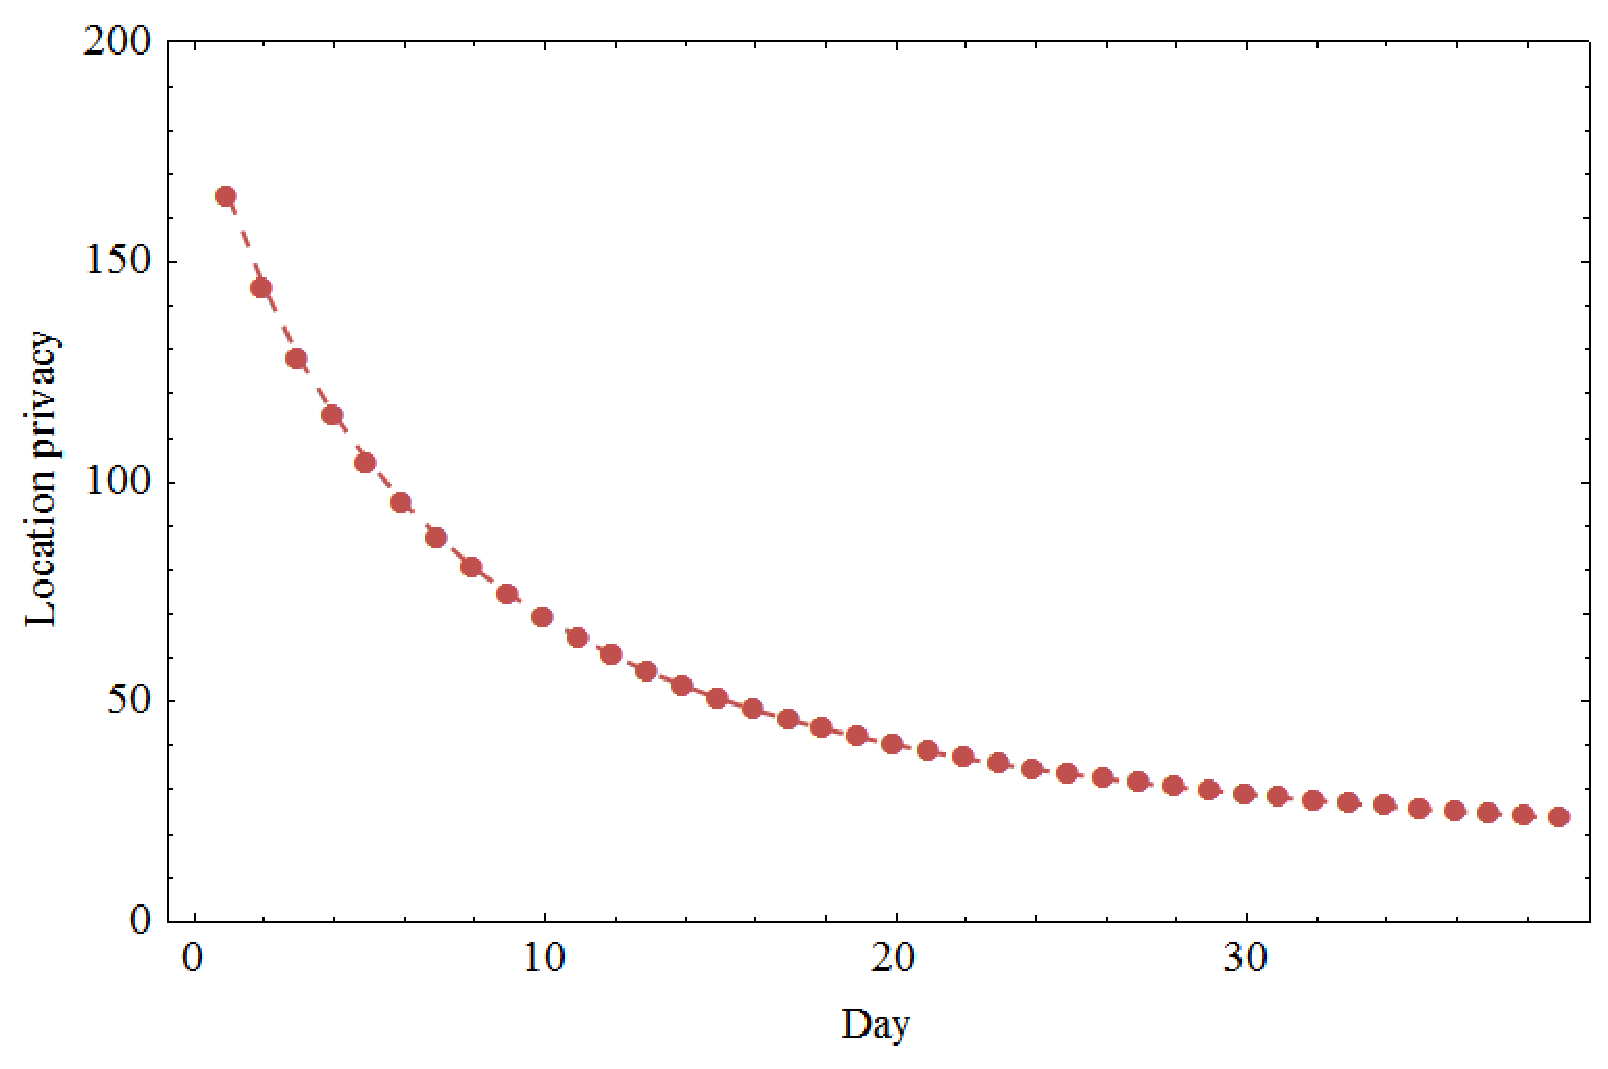
\includegraphics[width=0.55\textwidth]{chap4/exp1-su}
  \bicaption[fig:exp1-su]{认知用户的位置隐私泄露}{认知用户的位置隐私泄露}{Fig}{Location Privacy Leaking of Secondary Users}
\end{figure}

图\ref{fig:exp2-pu}展示了对主用户实施位置推断攻击的效果。可以看出,随着时间的增加,主用户的位置隐私泄露地更加明显,最终可能被攻击者锁定在5个小区域内,这个很高的定位精度源于数据库提供的丰富的而且细粒度的可用频谱信息。

\begin{figure}[!htp]
  \centering
  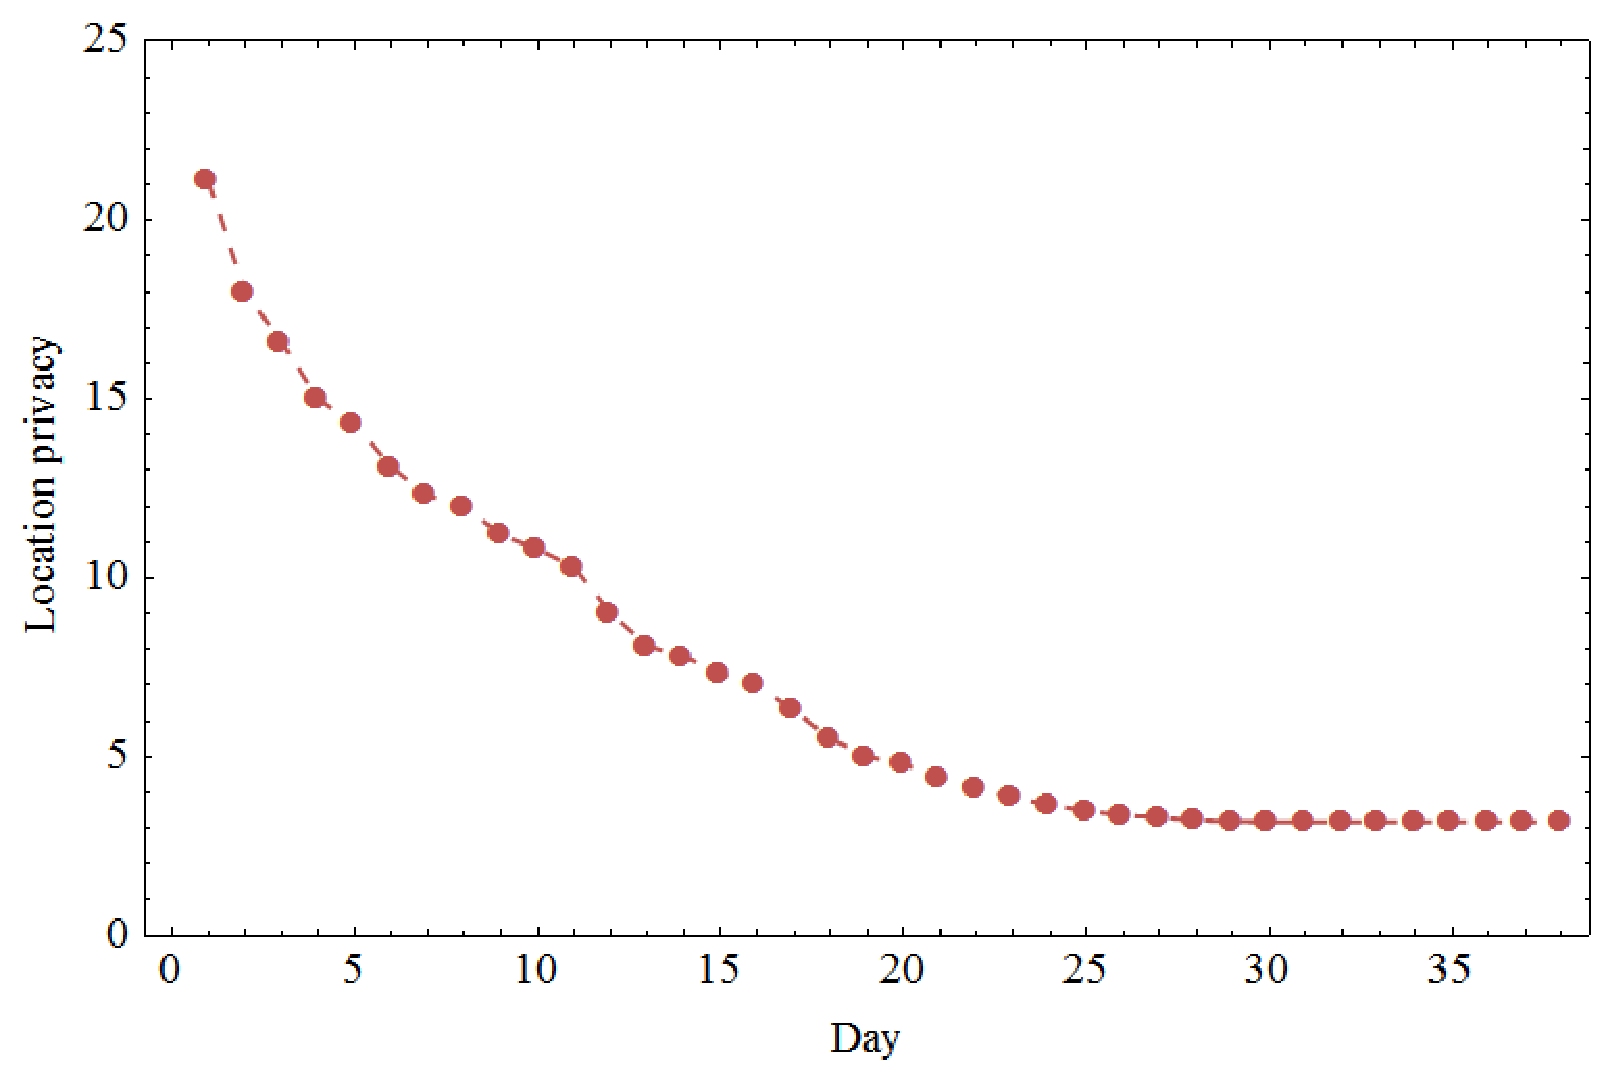
\includegraphics[width=0.55\textwidth]{chap4/exp2-pu}
  \bicaption[fig:exp2-pu]{主用户的位置隐私泄露}{主用户的位置隐私泄露}{Fig}{Location Privacy Leaking of Primary Users}
\end{figure}

我们对提出的隐私保护的可用频谱查询方案进行了实验验证,并与之前的查询方案进行了对比。在采用隐私保护的可用频谱查询前后,我们分别随机采样了若干认知用户来分析频谱效益和隐私保护。在图\ref{fig:exp3-su}中,标注random的曲线簇意味着随机选取接入频道,标注为optimal的曲线簇意味在文中提出的隐私保护框架下能够实现的最优结果。容易得知,在没有采用隐私保护措施时,认知用户即使在牺牲很多频谱效益的情况下也无法获得满意的隐私保护程度。若采用隐私保护的频谱选择策略,则认知用户理论上能够实现的隐私保护程度将大大提高,但无法避免由此带来的频谱效益的下降。

\begin{figure}[!htp]
  \centering
  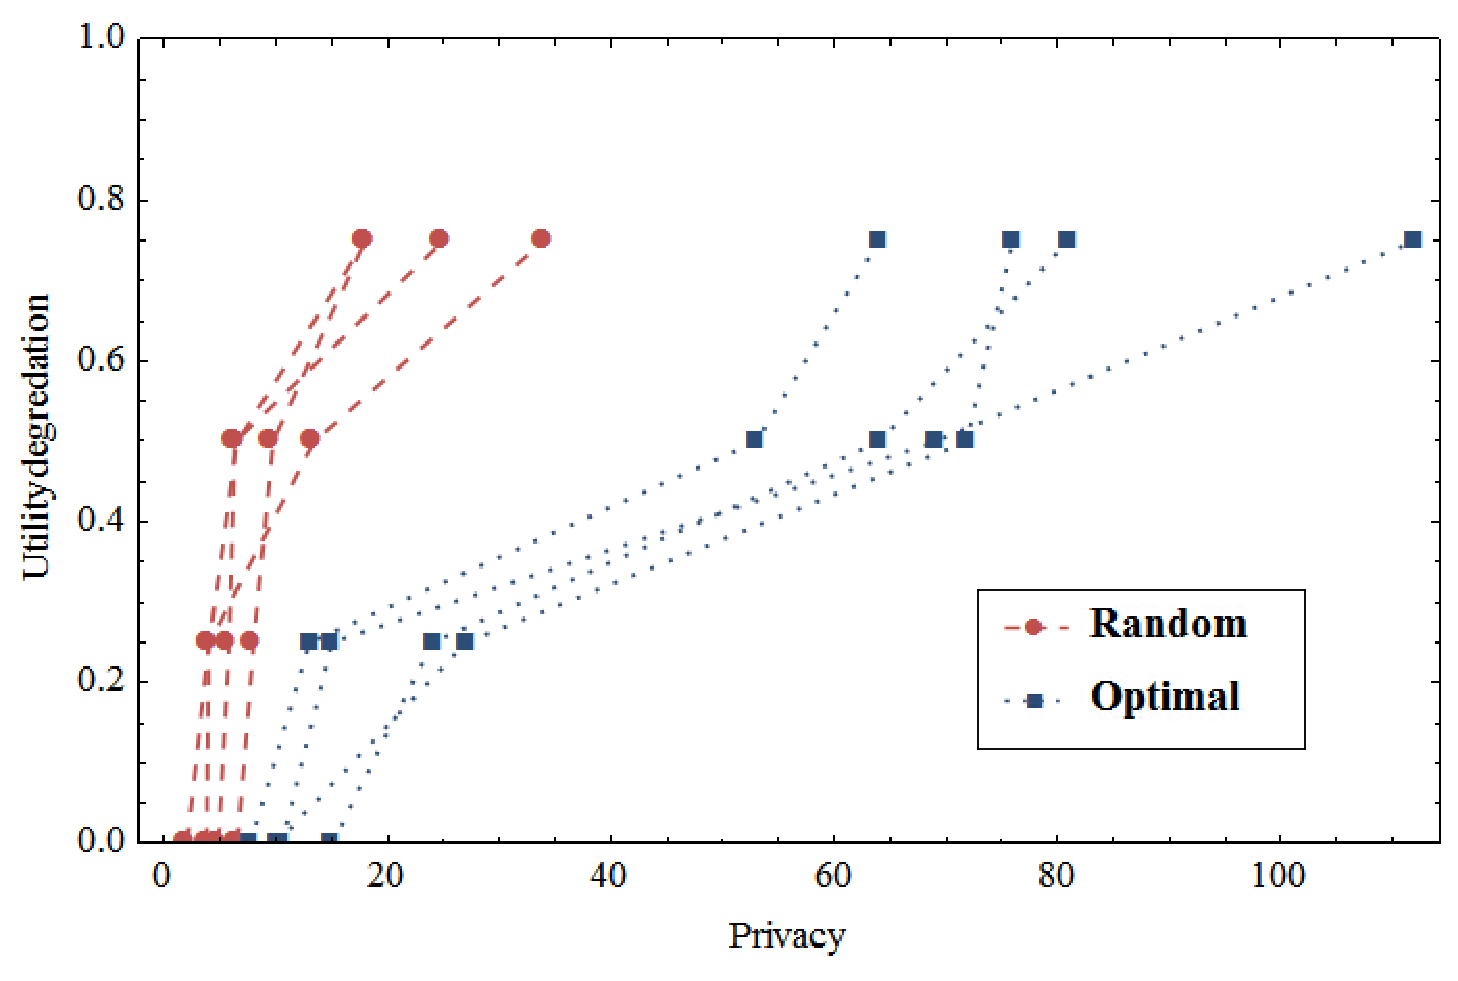
\includegraphics[width=0.6\textwidth]{chap4/exp3-su}
  \bicaption[fig:exp3-su]{认知用户的频谱效益与隐私}{认知用户频谱效益与隐私}{Fig}{Spectrum Utility and Location Privacy of Secondary Users}
\end{figure}

我们也分析了主用户采用隐私保护手段后的效果。在图\ref{fig:exp4-pu}中,标注为random的曲线意为数据库随机选择$K_{R}$的值来计算可用频谱,标注为optimal的曲线意为数据库在最优值的情况下能够达到的频谱效益和隐私保护的折中。我们可以看出,基于$k$-anonymity的频谱响应可以显著提高隐私保护程度,而且通过合理地选择$K_{R}$,我们还可以大大减少频谱效益的下降。

\begin{figure}[!htp]
  \centering
  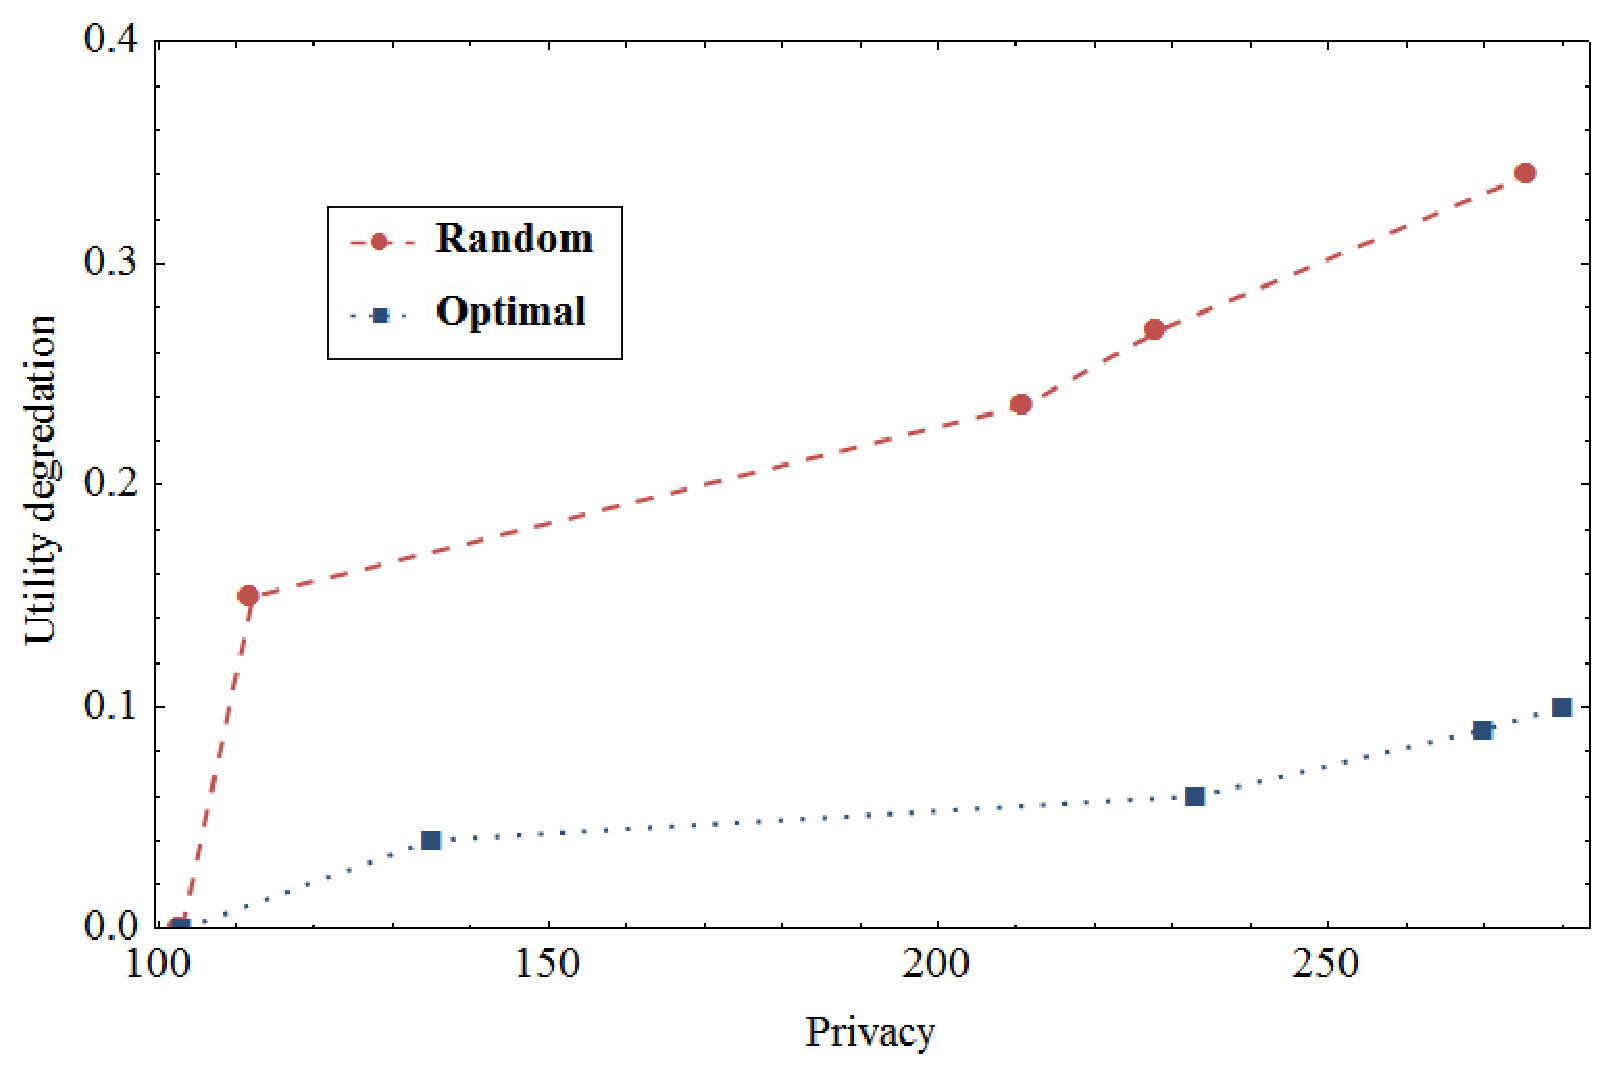
\includegraphics[width=0.6\textwidth]{chap4/exp4-pu}
  \bicaption[fig:exp4-pu]{数据库的频谱效益与隐私}{数据库的频谱效益与隐私}{Fig}{Spectrum Utility and Location Privacy of Primary Users}
\end{figure}

我们还可以预测,若认知用户选择了较大的$K_{Q}$值,则数据库会提供更多位置的频谱可用信息从而为认知用户选择使用频道提供详细的知识,但是更丰富的频谱可用信息也意味着主用户的隐私泄露更多,因此数据库反而可能会增大$K_{R}$的值来减少主用户隐私泄露,那么也相应导致数据库频谱效率的降低。由于认知用户在不清楚网络中主用户具体位置的前提下无法在本地确定隐私泄露的情况,而且动态调整$K_{Q}$和$K_{R}$的复杂度较高,所以本文没有对$K_{Q}$的取值对隐私保护的影响进行研究。


%%==================================================
%% chapter03.tex for SJTU Master Thesis
%% Encoding: UTF-8
%%==================================================

\chapter{数据库驱动认知无线电网络中的轨迹跟踪攻击与保护}
\label{chap:mobile}

\section{对认知用户轨迹跟踪攻击}
近年来研究者们发现,对于移动的用户,仅仅保护其位置隐私是不够的,因为对位置隐私的保护并不一定能够保证移动对象的轨迹隐私不被泄露。移动对象的原始轨迹暴露可能导致个人兴趣爱好以及行为模式等隐私信息泄露。比如,通过对轨迹数据的分析,攻击者不仅能够发现移动用户正在什么位置,还能够分析出移动对象的家庭住址、工作地点等私密信息。

在数据库驱动认知无线电网络中,静止用户之间的频谱共享能够较好地实现,但是当网络中存在移动用户时,如何较好地实现对主用户的保护以及如何根据移动用户位置计算频谱相关信息成为更具挑战性的问题\cite{min2011opportunistic}。文献\cite{gao2014supporting}提出一种基于概率的共存模型。数据库通过对认知用户之间的互相干扰来优化频谱分配方案,认知用户根据位置的不确定性对可能存在的干扰进行优化来确定位置更新的频率。然而无论采用何种共存模型,在可用频谱查询过程中,认知用户与数据库之间交互的信息都会导致轨迹隐私的泄露。本节对数据库驱动认知无线电网络中移动用户的轨迹隐私泄露及保护方法进行了研究。因为考虑到网络中的主用户大多为静止的,否则数据库计算频谱可用信息的复杂度将相当高,所以本节只考虑存在移动认知用户而主用户静止的情况下,攻击者对移动认知用户的轨迹跟踪攻击。


基于第\ref{chap:fixed}章的工作模型,我们依然假设认知用户采用了文献\cite{gao2013location}中的位置盲化方案,即在不直接获取认知用户的位置信息的前提下,对移动的认知用户轨迹进行跟踪。对移动用户的轨迹跟踪可以视为一个运动目标跟踪问题。目标跟踪问题中一种比较常用的是搜索方法。在搜索方法中,可以直接对场景中的所有内容进行匹配计算,寻找最佳匹配位置,但这种方法需要处理大量的冗余信息,运算量比较大并且不是特别必要。然而采用一定的搜索算法对未来时刻目标的位置状态进行估计假设,并指定搜索规则,则可以很大程度上缩小目标搜索范围,这具有非常重要的意义。比较常用的方法是预测运动物体下一时刻可能出现的位置,在其相关区域内寻找最优点。

递归贝叶斯估计是进行运动物体跟踪和预测的一种常用方法。递归贝叶斯估计方法\cite{bergman1999recursive}可用于估计隐马尔可夫模型中\cite{hmm}隐状态出现的概率。隐马尔可夫过程是一种统计模型,用来描述一个含有隐含未知参数的马尔可夫过程,其主要用途是从可观察的参数中确定该过程的隐含参数,然后利用这些参数来作进一步的分析,例如模式识别。图\ref{fig:hmm}简单描述了一个隐马尔可夫过程。


\begin{figure}[!htp]\label{fig:hmm}
  \centering
  \includegraphics[width=0.8\textwidth]{figures/chap5/hmm}\bicaption[fig:hmm]{隐马尔可夫模型}{隐马尔可夫模型}{Fig}{Hidden Markov Model}
\end{figure}

设$X=(x_{0},x_{1},...,x_{n})$是隐马尔可夫模型中的一系列隐状态,$Z=(z_{1},z_{2},...,z_{n})$表示一系列可观察状态。
设$Z_{k}$代表联合事件$z_{1},z_{2},...,z_{n}$。基于马尔可夫假设,隐马尔可夫过程中所有状态的概率分布可表示为:
\begin{equation}\label{eq:combination}
p(x_{0},...,x_{k},Z_{k})=p(x_{0})\prod_{i=1}^k{p(z_{i}|x_{i})p(x_{i}|x_{i-1})}
\end{equation}

基于公式\ref{eq:combination},我们可以将递归贝叶斯估计方法中的预测过程写为:
\begin{equation}\label{eq:predict}
p(x_{k}|Z_{k-1})=\int p(x_{k}|x_{k-1})p(x_{k-1}|Z_{k-1})dx_{k-1}
\end{equation}

将更新过程写为:
\begin{equation}\label{eq:update}
p(x_{k}|Z_{k})=\frac{p(z_{k}|x_{k})p(x_{k}|Z_{k-1})}{p(z_{k}|Z_{k-1})}
\end{equation}

为使用上述方法实现对隐状态的预测,我们需要计算$p_{z_{k}|x_{k}}$和$p(x_{k}|Z_{k-1})$两个概率。在对数据库驱动认知无线电网络中移动的认知用户进行轨迹跟踪时,隐状态$x_{i}$代表认知用户的移动轨迹,可观察状态$z_{i}$代表认知用户上报给数据库的使用频道和相应发射功率。我们需要为$x_{k}$与$z_{k}$以及$x_{k}$与$x_{k-1}$建立关联。连续两个隐状态之间的关联可由公式\ref{eq:hidden-states}表示:

\begin{equation}\label{eq:hidden-states}
x_{k}=f(x_{k-1})+v_{k}
\end{equation}

第$k$个时刻的隐状态和观察状态之间的关联可由公式\ref{eq:observed-states}表示:

\begin{equation}\label{eq:observed-states}
z_{k}=h(x_{k})+w_{k}
\end{equation}

这里的函数$f(\cdot)$和$h(\cdot)$是确定性函数,$v_{k}$和$w_{k}$是服从高斯分布的系统随机附加噪声。对移动认知用户的移动路线进行推断可以看成是一种目标跟踪问题。在目标跟踪问题里,$x_{k}$是目标移动信息,由位置$loc_{k}$和速度$vel_{k}$两个分量构成。前者为欧氏空间中的一个点,代表目标当前位置;后者为一个二维速度向量,表示当前目标速度值和运动方向。$z_{k}$代表认知用户接收到的可用频道和相应的允许发射功率,它是关于认知用户与主用户之间相对距离的函数,我们可以根据最大传输功率函数进行计算。

为描述$x_{k}$和$x_{k-1}$之间的关系,我们可以采用熟知的离散时间运动公式\cite{bar2004estimation}来表示:
\begin{equation}
x_{k}=F \cdot x_{k-1} + v_{k}
\end{equation}

在上式中,$F$为时间矩阵,可表示为:
\begin{equation}       %开始数学环境
F=
\left(                 %左括号
  \begin{array}{cc}   %该矩阵一共3列,每一列都居中放置
    1 & T\\  %第一行元素
    0 & 1\\  %第二行元素
  \end{array}
\right)                 %右括号
\end{equation}

$v_{k}=(v_{k}^{1},v_{k}^{2})^{T}$是加性的白噪声向量,其均值$E(v_{k})=0$,协方差矩阵为:
\begin{equation}
\sum = E(v_{k}v_{k}^{T})=
\left(                 %左括号
  \begin{array}{cc}   %该矩阵一共3列,每一列都居中放置
    \frac{1}{3}T^{3} & \frac{1}{2}T^{2}\\  %第一行元素
    \frac{1}{2}T^{2} & T\\  %第二行元素
  \end{array}
\right)                 %右括号
\sigma
\end{equation}

上式中$\sigma$是噪声强度,$T$是两次查询之间的时间间隔。因为考虑到函数$f(\cdot)$和$h(\cdot)$不是线性函数,因此我们采用粒子滤波(Particle Filter)\cite{arulampalam2002tutorial}方法来进行目标跟踪。

粒子滤波是指通过寻找一组在状态空间中传播的随机样本来近似的表示概率密度,用样本的均值代替积分运算,进而获得系统状态的最小方差估计的过程。粒子滤波算法起源于蒙特卡罗方法\cite{hastings1970monte},它是利用粒子集来表示概率分布,可以用在任意形式状态空间模型上,核心思想是通过从后验概率中抽取的随机状态粒子来表示其分布情况,是一种顺序重要性采样法。我们参照文献\cite{bahrak2013ex}提出的粒子滤波方案,在数据库驱动认知无线电环境中设计一种基本的跟踪移动认知用户的算法,其详细步骤见算法\ref{alg:pf}。

\begin{lstlisting}[language={C}, caption={基于粒子滤波的移动用户轨迹跟踪算法}]
输入:认知用户的频谱使用记录S=$(ch_{1},P_{1}),(ch_{2},P_{2}),...,(ch_{k},P_{k})$
输出:认知用户的轨迹信息,包含位置和速度
初始化:设定粒子数量$N_{P}$及初始权值
    
for 所有N_{P}个粒子$i$
    $\omega_{0}^{i}=\frac{1}{N_{P}}$
k=1
while 没有到达预先设定的终止条件 do
    观察到第$k$次事件:$(ch_{i}^{k},P_{i}^{k})$
    T = 第$k$次事件与第$k-1$次事件之间的时间间隔
    重采样:
      根据粒子的权值$\omega_{1},...,\omega_{N_{P}}$进行重要性采样
       依概率序列$(\omega_{k-1}^{1},\omega_{k-1}^{2},...,\omega_{k-1}^{N_{P}})$从粒子序列中采样,重复$N_{P}$次
    预测:
      for 所有的粒子$Par_{1},...,Par_{N_{P}}$ do
           计算运动信息$x_{k}^{i}$:
           $loc_{k}^{i} = loc_{k-1}^{i} + T \times vel_{k-1}^{i} + v_{k}^{1}$
           $vel_{k}^{i} = vel_{k-1}^{i} + v_{k}^{2}$
           $x_{k}^{i} = (loc_{k}^{i},vel_{k}^{i})$
       end for
    更新:
      for 所有的粒子$Par_{1},...,Par_{N_{P}}$ do
           计算粒子权值:
           $\omega_{k}^{i}=Pr(z_{k}|x_{k}^{i})$ = 
           $
           \begin{cases}
           0  \quad z_{k} \neq h(x_{k}^{i})\\
           1  \quad z_{k} = h(x_{k}^{i})
           \end{cases}
           $  
        end for
     粒子权值归一化:
       $\omega_{k}^{i} = \frac{\omega_{k}^{i}}{\sum_{i=1}^{N} \omega_{k}^{i}}$
end while
              
\end{lstlisting}\label{alg:pf}

在算法\ref{alg:pf}中,我们在初始化时使用一个包含有足够多随机分布的粒子来对移动认知用户的位置及速度信息进行估计。在粒子滤波的过程中,每一轮分为重采样、预测和更新三个步骤。重采样时根据上一轮更新步骤中计算出的各粒子的权值进行重要性采样,即只在权值不为0的粒子周边进行采样。在预测阶段,根据预先猜测的粒子运动信息的大致情况来对各粒子的位置和速度进行估算。在更新阶段,若粒子位置符合当前上报的可用频谱单元,则将其权值更新为1,否则权值更新为0。最后将所有粒子的权值进行归一化并用于下一轮的重采样。具体地讲,假设从后验概率$Pr(x_{k-1}|Z_{k-1})$中随机采样$N_{P}$个粒子,我们将这些粒子表示为$\hat{x}_{k-1}^{i},1 \leq i \leq N$。在预测阶段,根据公式\ref{eq:hidden-states}在后验粒子$\hat{x}_{k-1}^{i}$的基础上生成先验粒子$x_{k}^{i}$,即

\begin{equation}
x_{k}^{i} = f_{k-1}(\hat{x}_{k-1}^{i}) + v_{k-1}^{i}
\end{equation}

这里$v_{k-1}^{i}$表示从系统噪声的概率分布中随机抽取的样本。这个过程相当于从创建了先验概率$Pr(x_{k}|Z_{k-1})$中的采样。为了使用观察状态$z_{k}$对粒子状态进行更新,我们为每个粒子计算权值$\tilde{\omega}_{k}^{i}$。这个权值是观察状态的似然,即

\begin{equation}
\tilde{\omega}_{k}^{i} = Pr(z_{k}|x_{k}^{i})
\end{equation}

然后权值需要进行归一化,即
\begin{equation}
\omega_{k}^{i} = \frac{\tilde{\omega}_{k}^{i}}{\sum_{j=1}^{N}\tilde{\omega}_{k}^{i}}
\end{equation}

基于每个粒子的归一化权值,在下一轮重采样时根据相应的权值来创建新的粒子集$\hat{x}_{k}^{i}$,使得对于所有的$i,j$,满足$Pr(\hat{x}_{k}^{i} = x_{k}^{i}) = \omega_{k}^{j}$。
也就是说,每一次采样都是根据粒子的归一化概率进行的,将此过程重复$N_{P}$次,即完成了$N_{P}$个粒子的重采样。

在实际情况下,按照FCC的规定,移动用户每次移动超过100米,则必须要重新查询可用频谱情况以避免对主用户产生干扰,持续移动的认知用户必将频繁地查询数据库。因此以上算法在用户不断移动时能够收集足够多的频谱使用报告消息来实施攻击。

\section{轨迹跟踪攻击的解决方案}

在传统的LBS中,第\ref{chap:related_work}章所述的几种方法一般能够取得一定效果。但是数据库驱动认知无线电网络中用户轨迹跟踪问题与传统的基于位置服务网络中轨迹跟踪问题不同,好奇的数据库可以以频谱使用信息这类旁道信息作为依据来实施推理,而且数据库驱动认知无线电网络中的用户身份标识在注册后无法改变,因此如何防止轨迹跟踪成为一个具有挑战性的问题。在静止认知用户的位置推断攻击中,我们总结了两种导致隐私泄露发生的事件:功率受限和频道切换。移动的用户面临与之相似的泄露方式但却不完全相同。为尽量保护移动用户的轨迹隐私不被泄露,我们仍然将重点放在如何提高攻击者攻击结果的误差距离上面。下面我们考虑如下几种可能发生的情况。

\begin{enumerate}

\item 若某个时刻用户使用频道的功率受限,则可以推断此刻认知用户的位置范围大致在一个圆环型区域,从而在下一轮采样时可根据重要性的变化从而对可能区域周边进行重点采样。这种情况可以导致对跟踪目标运动信息不确定性减小。

\item 若某两个连续的频谱报告消息中频道相同,但允许发射功率变大,则用户持续使用该频道不会导致轨迹信息泄露。若频道相同且发射功率变小,则会面临与功率受限相同的隐私泄露风险。

\item 若某两个连续的频谱报告中认知用户切换了频道,由于相邻两次查询之间认知用户移动的距离不会太远,则攻击者可以在很大程度上认定认知用户处于两个频道的相应功率覆盖范围的交集区域,这也会导致运动信息不确定性减小。

\item 若一个认知用户在其移动范围内可以一直使用一个固定的频道而且该频道的允许发射功率不变,那么针对上一节提出的攻击方法,我们可以通过选择最合适的频道来在最大程度上减小认知用户轨迹信息的泄露。

\end{enumerate}

根据以上分析,我们可以知道,最好的情况是认知用户能够在其移动的轨迹上持续使用相同的频道,且允许发射功率越大越好。于是我们提出如下的频谱查询和选择策略:

(1)在可用频谱请求阶段,用户采用第\ref{subsec:privacy-preserving}节提出的基于$k$-anonymity的查询方式,即同时查询周边大小为$K_{Q} \times K_{Q}$的区域$B$上的可用频谱信息。在接下来的频道选择阶段,认知用户可以根据这些信息来选择在其移动轨迹上最优的频道。

(2)在频谱选择阶段,用户维护一个关于所有频道的优先级列表:$U=(u_{1},u_{2},...,u_{C})$,每个频道$ch_{k}$的优先级可以表示为:

\begin{equation}
u_{k} = \sum_{c \in B} P_{k}^{c}
\end{equation}

即所有查询区域中的功率等级的总和。用户应该选择优先级最高的频道使用。在不断移动和查询的过程中,当用户发现其正在使用的频道优先级低于某个其他频道时,若原来使用的频道功率等级最高,则不切换频道;否则应切换到新发现的最高优先级的频道。频道优先级的值比较大则说明用户在可预计的范围$B$内移动时,有很高的概率可以持续使用该频道而不用切换,从而能够减少轨迹隐私的泄露。尽管可能会由于主用户上线而导致频道切换,认知用户还是可以通过选择其他高优先级的频道来尽可能保护隐私。

\section{轨迹跟踪攻击和隐私保护方案验证}

为验证上文提出的攻击以及隐私保护方案的有效性,我们基于模拟数据进行了实验验证。假设数据库管理一个$50km \times 50km$的正方形区域,该区域划分为$500 \times 500$个$100m \times 100m$的小正方形区域。整个区域中随机分布20个主用户,主用户随机切换在线/离线状态。我们仍然采用公式\ref{eq:coverage}所示的MTP函数。假定认知用户的移动速度不会太快,最高速度不超过80km/h。在移动过程中,认知用户随机选择接入的频道。图\ref{fig:particles}展示了对一个沿直线移动的认知用户的跟踪过程。

\begin{figure}
\centering
\subfigure[5次查询后]
{
\begin{minipage}[b]{0.45\textwidth}
  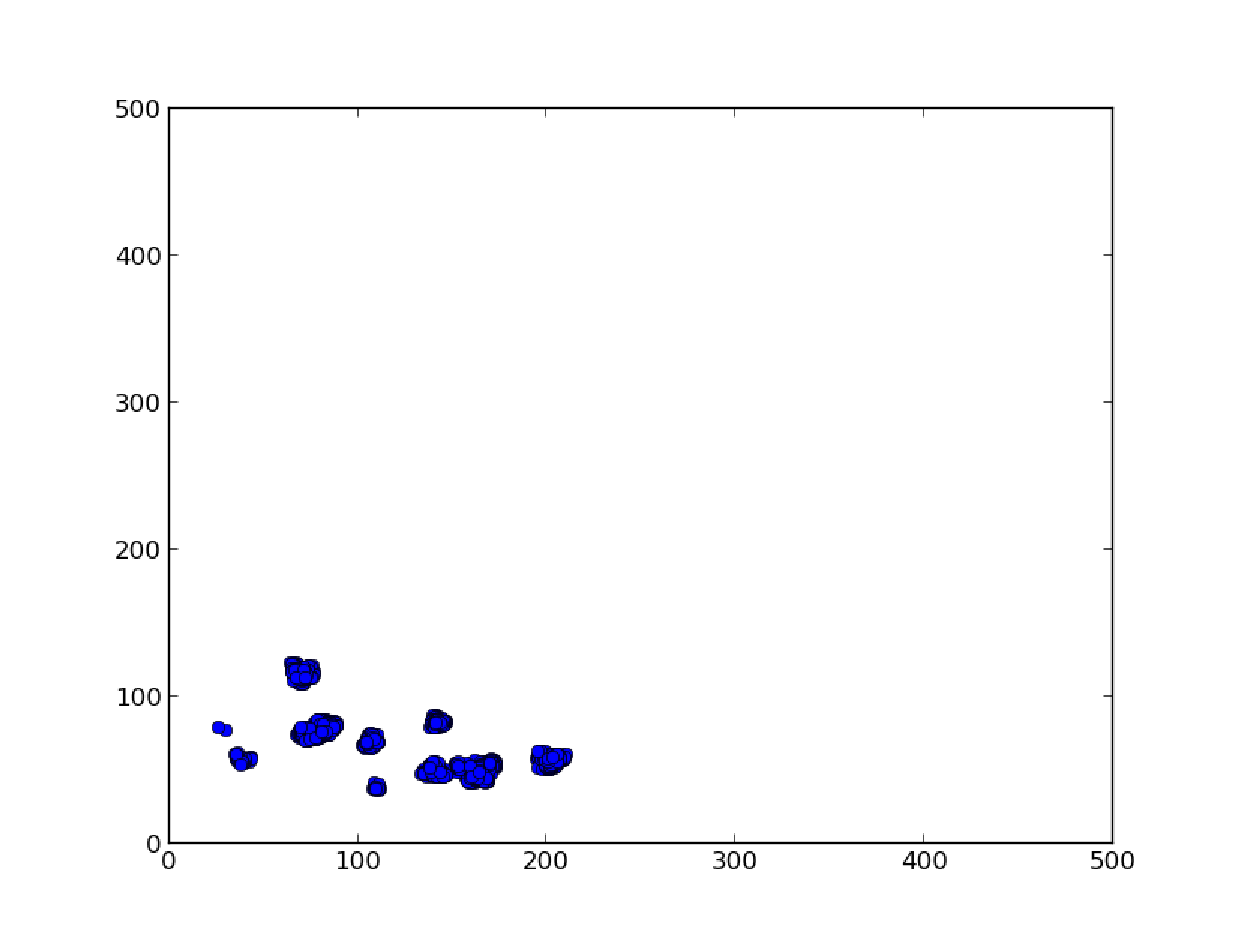
\includegraphics[width=0.9\textwidth]{figures/chap5/attack-mobile-5iterations.eps}\label{fig:mobile-5queries}
\end{minipage}
}
\hfill
\subfigure[10次查询后]
{
\begin{minipage}[b]{0.45\textwidth}
  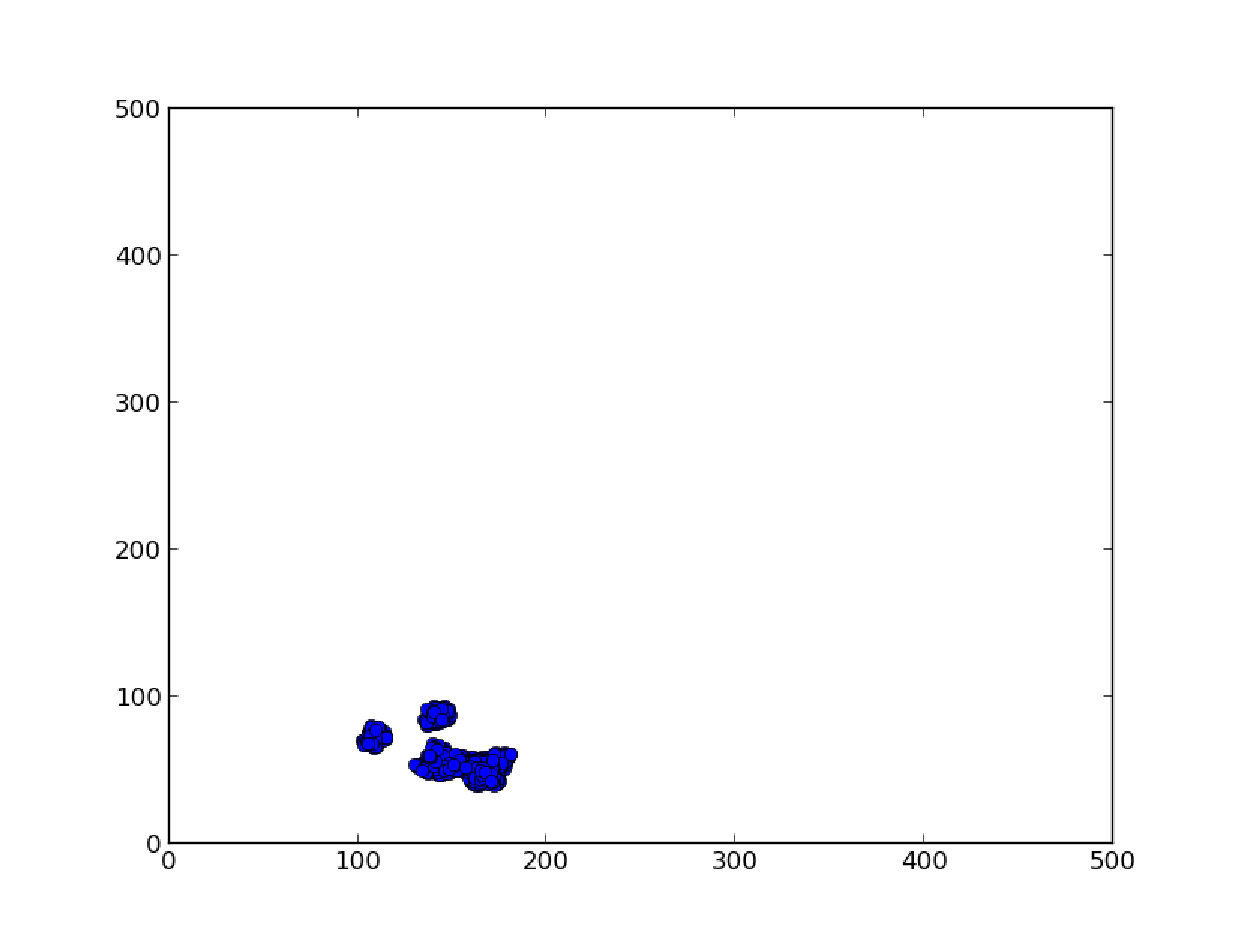
\includegraphics[width=0.9\textwidth]{figures/chap5/attack-mobile-10iterations.eps}\label{fig:mobile-10queries}
\end{minipage}
}

\subfigure[15次查询后]
{
\begin{minipage}[b]{0.45\textwidth}
  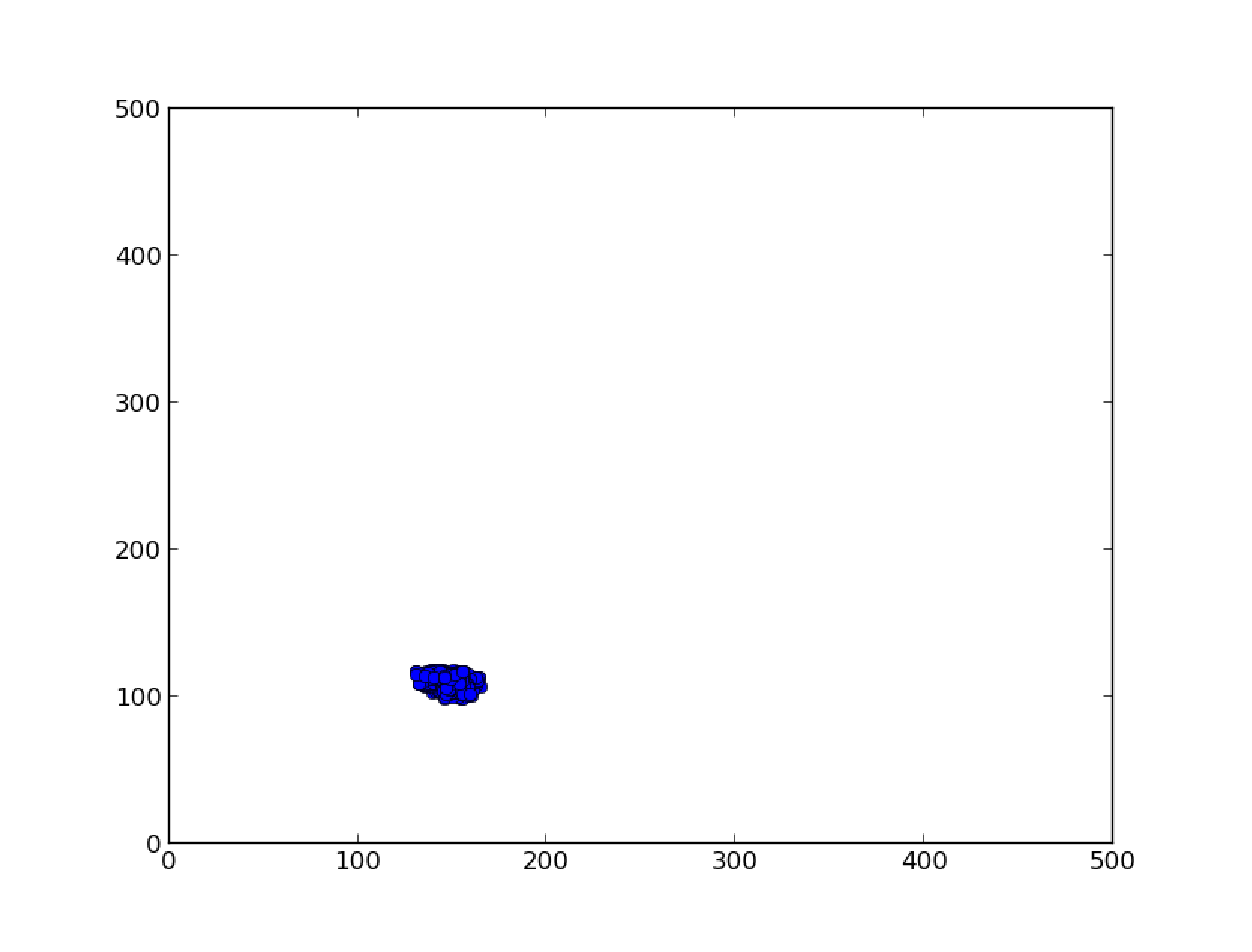
\includegraphics[width=0.9\textwidth]{figures/chap5/attack-mobile-15iterations.eps}\label{fig:mobile-15queries}
\end{minipage}
}
\hfill
\subfigure[20次查询后]
{
\begin{minipage}[b]{0.45\textwidth}
  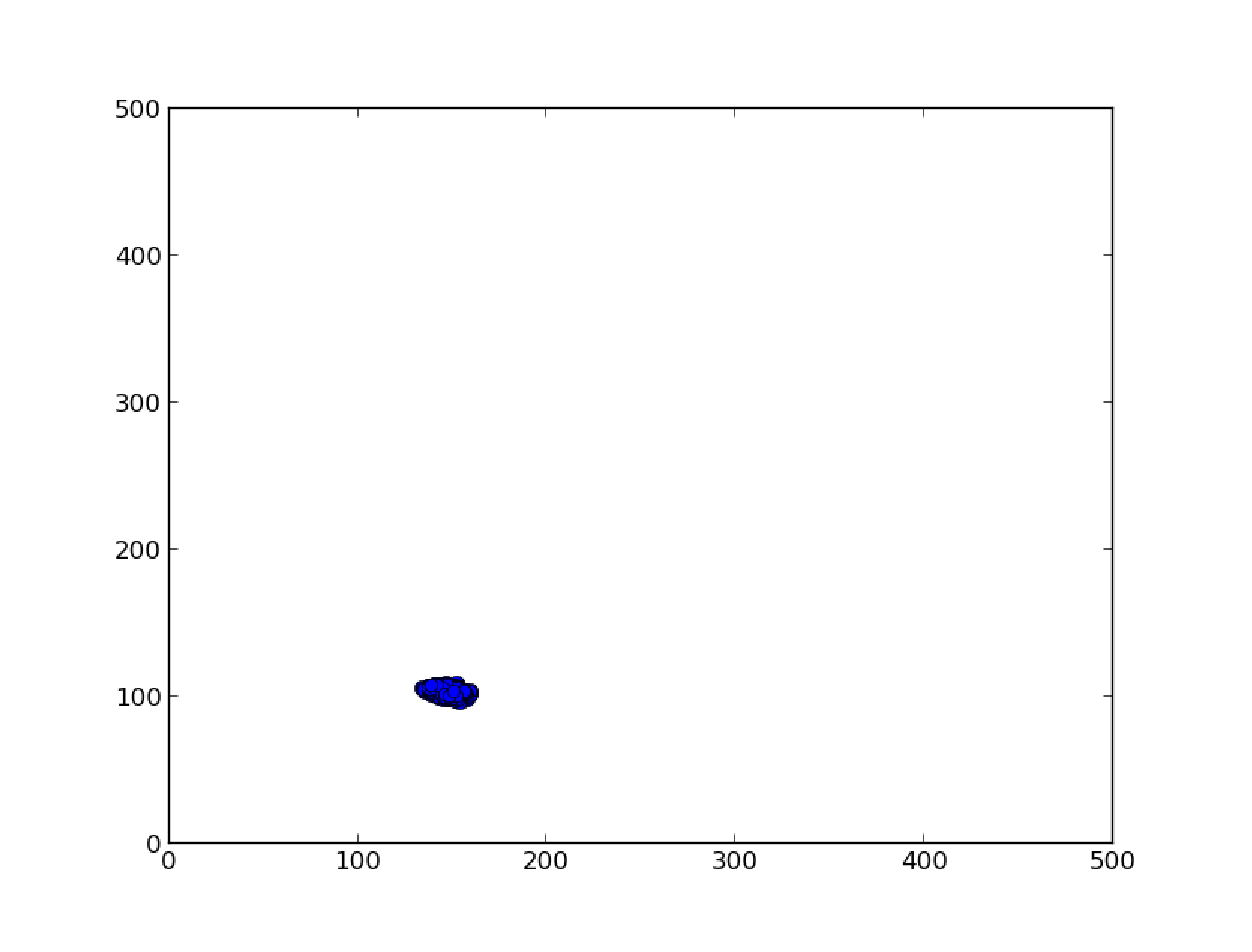
\includegraphics[width=0.9\textwidth]{figures/chap5/attack-mobile-20iterations.eps}\label{fig:mobile-20queries}
\end{minipage}
}
\caption{跟踪过程中的粒子位置状态}\label{fig:particles}
\end{figure}

一般情况下,我们仅通过20次查询即可将移动的认知用户位置锁定在较小的区域范围内。进一步,为了衡量跟踪的准确程度,我们采用第\ref{chap:fixed}章提出的平均误差距离的概念来对文中提出的跟踪算法进行准确性的描述。我们对几种不同的运动形式包括直线运动、一般形式的曲线运动、以及随机游动分别进行了对比,如图\ref{fig:diverse-pattern}所示。其中实验结果表明,我们提出的算法对几种不同的运动方式都有比较好的跟踪精确度,而且对于不同运动状态的移动用户的跟踪结果相差无几。随着时间以及查询次数的增加,对目标认知用户的跟踪精度也逐渐增加。

\begin{figure}[!htp]\label{fig:diverse-pattern}
  \centering
  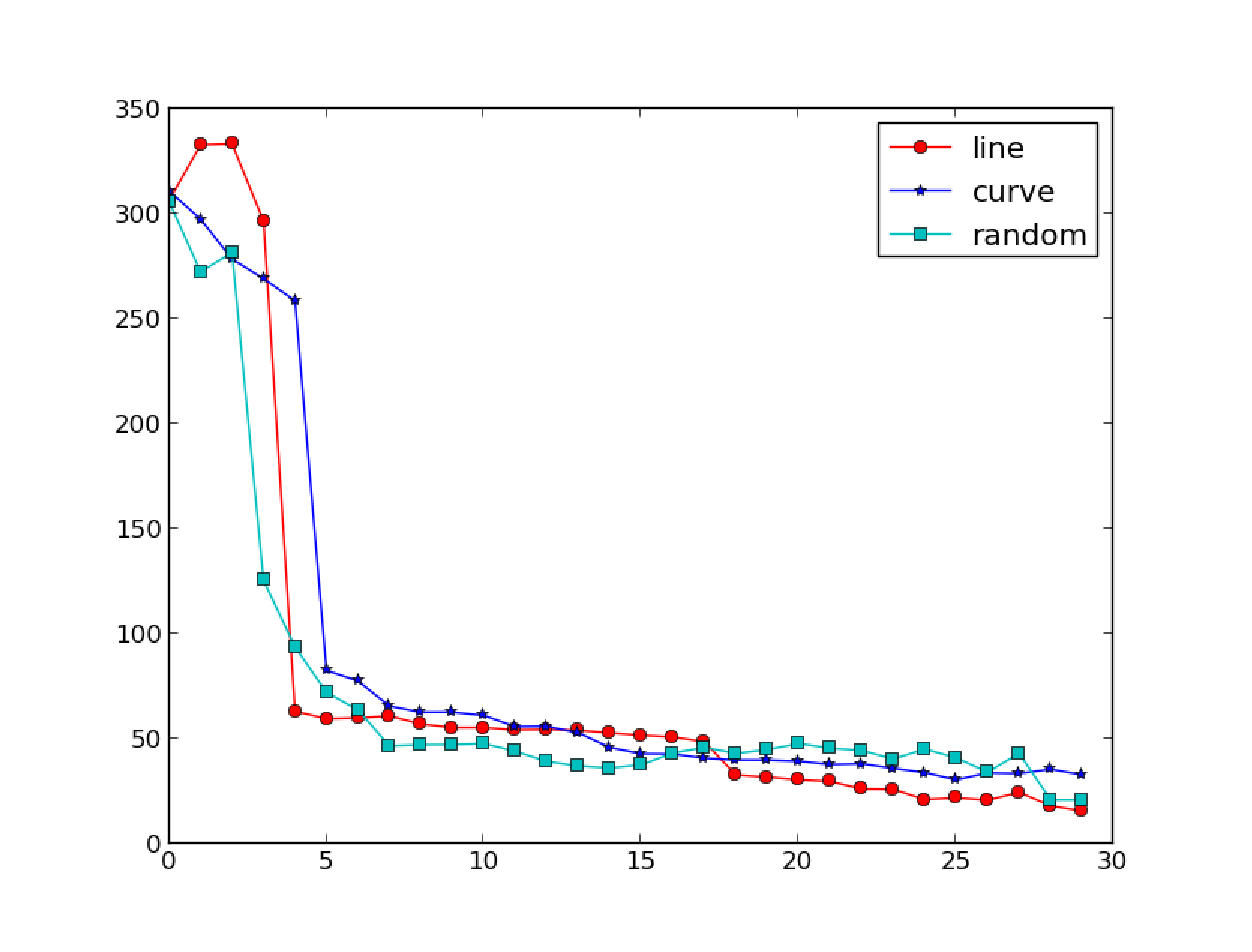
\includegraphics[width=0.7\textwidth]{figures/chap5/diversity}\bicaption[fig:diverse-pattern]{对不同运动形式用户的跟踪结果}{对不同运动形式用户的跟踪结果}{Fig}{Tracking Results on Mobile Users of Different Patterns}
\end{figure}

为检验提出的隐私保护的频谱查询和使用方案的有效性,我们对20组实验数据进行了统计,每一次实验随机生成主用户的位置并随机设置认知用户的移动轨迹。我们将采用隐私保护频谱查询和选择方案前后的跟踪误差进行了对比,如图\ref{fig:countermeasure}所示。容易看出,在使用隐私保护的频谱查询和选择方案后,由于认知用户在运动过程中尽可能选择功率大且覆盖范围广的频谱资源,而且尽量减少不必要的频道切换,导致
攻击者在短期内几乎无法通过本文提出的算法实现跟踪,攻击效率大幅度下降。

\begin{figure}[!htp]\label{fig:countermeasure}
  \centering
  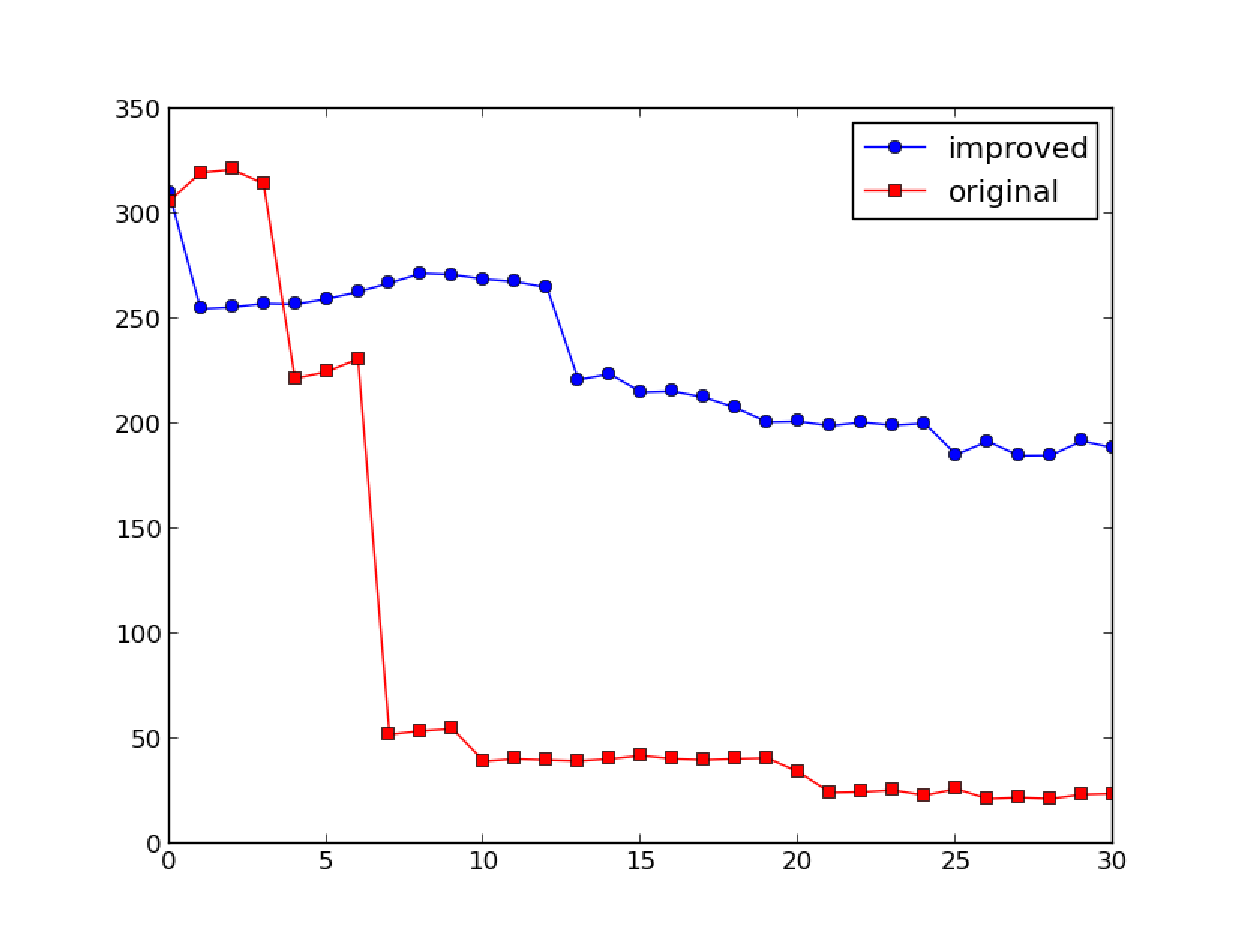
\includegraphics[width=0.7\textwidth]{figures/chap5/countermeasure}\bicaption[fig:countermeasure]{隐私保护的查询和选择方案的性能}{隐私保护的查询和选择方案的性能}{Fig}{Performance of Privacy Preserving Spectrum Query and Selection Scheme}
\end{figure}
%%==================================================
%% conclusion.tex for SJTU Master Thesis
%% based on CASthesis
%% modified by wei.jianwen@gmail.com
%% version: 0.3a
%% Encoding: UTF-8
%% last update: Dec 5th, 2010
%%==================================================

\chapter*{全文总结\markboth{全文总结}{}}
\addcontentsline{toc}{chapter}{全文总结}

这里是全文总结内容。
本文论述了数据库驱动认知无线电网络中的用户位置隐私和轨迹隐私的攻击和保护的问题。本文的主要内容包括:

\begin{enumerate}

\item 提出了数据库驱动认知无线电网络中静止用户的位置隐私泄露的问题。根据频谱信息与用户位置的相关性,实现了对静止用户的位置推断攻击并提出了相应的解决方案。通过选择合适的参数和策略,认知用户和主用户能够显著提高其位置隐私保护程度。

\item 基于频谱信息与用户位置的相关性,提出了对移动认知用户的轨迹跟踪方案,通过对认知用户上报的通知信息进行相似性匹配从而实现了用户运动信息的估计。进一步提出了能够应对轨迹跟踪攻击的隐私保护的频谱查询和选择方案,很大程度上提高了移动认知用户的轨迹隐私保护。

\end{enumerate}

本文主要关注数据库驱动认知无线电网络中的位置与轨迹隐私方面的问题并提出了攻击和解决方案。数据库驱动认知无线电网络的概念提出的时间不久,随着其关注度的逐渐提高,其中的安全和隐私等相关问题也必将成为一个重要的研究方向。 %% 全文总结


%%%%%%%%%%%%%%%%%%%%%%%%%%%%%% 
%% 附录(章节编号重新计算,使用字母进行编号)
%%%%%%%%%%%%%%%%%%%%%%%%%%%%%% 
\appendix

% 附录中编号形式是"A-1"的样子
\renewcommand\theequation{\Alph{chapter}--\arabic{equation}}
\renewcommand\thefigure{\Alph{chapter}--\arabic{figure}}
\renewcommand\thetable{\Alph{chapter}--\arabic{table}}

%%==================================================
%% app1.tex for SJTU Master Thesis
%% based on CASthesis
%% modified by wei.jianwen@gmail.com
%% version: 0.3a
%% Encoding: UTF-8
%% last update: Dec 5th, 2010
%%==================================================

\chapter{基于私有信息提取的查询盲化方案}
\label{chap:updatelog}

在数据库驱动认知无线电网络中,假设数据库管理的区域为$C$,每个区域划分为若干小区域,表示为$c_{ij}$。数据库在区域$C$上通过计算得到的频谱信息数据库表示为$M$,每个区域$c_{ij}$对应的可用频谱信息表示为$m_{ij}$。认知用户进行可用频谱信息请求时,关心$m_{ij}$的内容,但是想要将$i$和$j$保密。基于私有信息提取的查询盲化方案如下:

\begin{enumerate}

\item 初始化:

首先认知用户在本地生成一个大素数$p$和两个随机数$b,d$,$b,d$作为请求过程中的盲化因子。计算$b^{-1}$和$d^{-1}$。然后生成两个随机向量$\vec v_{1} = (a_{1},a_{2},...,a_{n})$和$\vec v_{2} = (c_{1},c_{2},...,c_{n})$,向量中的元素需要满足:

\begin{displaymath}
a_{i},c_{i} < \frac{\sqrt{p}-\sqrt{N-1}}{nN\sqrt{N-1}},1 \leq i \leq n
\end{displaymath}

式中,$n$是可用频谱信息矩阵向量的维数;$N=2^{K}$,$K$为频道数量。

\item 查询信息盲化:

认知用户对$\vec v_{1}$和$\vec v_{2}$按照如下方式进行处理:
\begin{displaymath}
\vec v_{1}' = (a_{1}',a_{2}',...,a_{n}')=N \cdot \vec v_{1}' + \vec h_{i} = (a_{1}N,...,a_{i}N+1,...,a_{n}N)
\end{displaymath}

\begin{displaymath}
\vec v_{2}' = (c_{1}',c_{2}',...,c_{n}')=N \cdot \vec v_{2}' + \vec h_{j} = (c_{1}N,...,c_{j}N+1,...,c_{n}N)
\end{displaymath}

式中$\vec h_{i},\vec h_{j}$是单位向量,向量的第$j$或$j$个元素为1,其他元素全部为0。为隐藏$\vec v_{1}$和$\vec v_{2}$的真实值,认知用户使用盲化因子$b$和$d$分别对$\vec v_{1}'$和$\vec v_{2}'$进行处理如下:

\begin{displaymath}
\vec u_{1} = b \cdot \vec v_{1}' \ mod p = (ba_{1}N,...,b(a_{i}N+1),...,ba_{n}N) \ mod p
\end{displaymath}

\begin{displaymath}
\vec u_{2} = d \cdot \vec v_{2}' \ mod p = (dc_{1}N,...,d(c_{i}N+1),...,dc_{n}N) \ mod p
\end{displaymath}
然后认知用户向数据库发送查询消$Q=(\vec u_{1},\vec u_{2})$。

\item 查询执行:
数据库在收到查询消息$Q$之后,首先计算查询结果$g = \vec u_{1} \cdot M \cdot \vec u_{2}^{T}$,此时不需要进行模运算。式中$\vec u_{2}^{T}$是$\vec u_{2}$的转置。然后数据库将$g$作为响应消息发给认知用户。这个操作与直接传输可用频谱信息矩阵$M$在很大程度上能够减小传输开销。

\item 结果恢复:
为恢复可用频谱信息,认知用户计算$g_{1} = b^{-1} \cdot g \cdot d^{-1}$,因而而频谱可用信息$m_{ij}=g_{1} \ mod p \ mod N$。

\end{enumerate}
 % 更新记录

% \include{body/app3}


%%%%%%%%%%%%%%%%%%%%%%%%%%%%%% 
%% 文后(无章节编号)
%%%%%%%%%%%%%%%%%%%%%%%%%%%%%% 
\backmatter

% 参考文献
% 使用 BibTeX
% 包含参考文献文件.bib
\bibliography{reference/bibliography}

%% 个人简历(硕士学位论文没有个人简历要求)
% \include{body/resume}

% 致谢
%%==================================================
%% thanks.tex for SJTU Master Thesis
%% based on CASthesis
%% modified by wei.jianwen@gmail.com
%% version: 0.3a
%% Encoding: UTF-8
%% last update: Dec 5th, 2010
%%==================================================

\begin{thanks}

在我攻读硕士学位的这不到三年的时间里,有很多老师、同学和朋友们给了我真诚的帮助和指导,才使我能够愉快地度过研究生阶段生活并顺利地完成学业。在本论文即将完成之际,谨向他们表达我最诚挚的感谢。

首先要感谢我的导师--朱浩瑾老师,在攻读硕士期间,他无论是在科研工作还是日常生活方面都给了我无微不至的指导和关心。在撰写论文的全过程,包括选题、资料搜集、文章结构组织、语言表达乃至很多细节的方面,他都对我进行了详细的指导。此外,他不但具有广播的学识和一丝不苟的科研态度,还有着令人敬仰的无限人格魅力,他对我的潜移默化的影响也将是我一生的财富。

同时我还要感谢学弟方晨廖晖,他凭借扎实的代码功底在我论文的实验部分给予了大量帮助。感谢NSEC实验室和所有实验室里的师兄师弟们,感谢他们陪伴我度过了人生中很美好的一段时光,也感谢他们对我平时工作生活中的无私的帮助。

最后我要感谢我的爱人,他对我一如既往的支持和鼓励一直是我努力工作的动力。

由于学术水平有限,我的论文难免有不足之处,恳请各位老师和学友批评和指正!
  

\end{thanks}


% 发表文章目录
%%==================================================
%% pub.tex for SJTU Master Thesis
%% based on CASthesis
%% modified by wei.jianwen@gmail.com
%% version: 0.3a
%% Encoding: UTF-8
%% last update: Dec 5th, 2010
%%==================================================

\begin{publications}{99}

    \item\textsc{张龙, 高昭瑜, 朱浩瑾, 等}. {数据库驱动认知无线电网络位置隐私的攻击与保护}[J]. 中国科技论文, 2014, 9(7): 754-757.
     
\end{publications}





% 参与项目列表
%%==================================================
%% projects.tex for SJTU Master Thesis
%% based on CASthesis
%% modified by wei.jianwen@gmail.com
%% version: 0.3a
%% Encoding: UTF-8
%% last update: Dec 5th, 2010
%%==================================================

\begin{projects}{99}

    \item 自然基金项目“认知无线电网络合作频谱感知中的安全与隐私问题研究“ 
    
\end{projects}


\end{document}
